\documentclass{article}
\usepackage{geometry}
\usepackage[normalem]{ulem}

\geometry{a4paper, lmargin=2cm, rmargin=3cm, tmargin=2cm, bmargin=2cm}
\usepackage{amsmath, amssymb, amsthm}
% \usepackage[margin=1in]{geometry}
\usepackage{tikz}
\usepackage{booktabs}

\usetikzlibrary{shapes.geometric}
\usepackage{ifthen,array,xcolor,colortbl,caption,subcaption,graphicx}
\usetikzlibrary{arrows.meta, positioning, shapes.geometric}
\usepackage{parskip}
\usepackage{matlab-prettifier}
\usepackage{listings}
\lstdefinestyle{mystyle}{
    backgroundcolor=\color{white},   
    commentstyle=\color{green},
    keywordstyle=\color{magenta},
    numberstyle=\tiny\color{teal},
    stringstyle=\color{teal},
    basicstyle=\ttfamily\color{teal}
    }
\lstset{style=mystyle}
\setlength{\parindent}{1.5em}

% ---------- colours ----------
\definecolor{headergray}{gray}{0.90}
\definecolor{starfill}{RGB}{45,45,55}   % dark star; try {RGB}{240,180,40} for gold

%For hyperlinks
\usepackage[normalem]{ulem}
\usepackage{hyperref}
\hypersetup{
	pdfborder={0 0 0},
	colorlinks,
	linkcolor={red!50!black},
	citecolor={blue!50!black},
	urlcolor={blue!80!black},
}
\newcommand{\myhref}[2]{\href{#1}{\uline{#2}}}


%Environments
\newtheorem{theorem}{Theorem}[section]
\newtheorem{cor}[theorem]{Corollary}
\newtheorem{lemma}[theorem]{Lemma}
\newtheorem{prop}[theorem]{Proposition}
\theoremstyle{definition}
\newtheorem{definition}[theorem]{Definition}
\newtheorem{algorithm}[theorem]{Algorithm}
\theoremstyle{remark}
\newtheorem{remark}[theorem]{Remark}
\newtheorem{conj}[theorem]{Conjecture}
\numberwithin{equation}{section}

%Commands
\newcommand{\bA}{\mathbf{A}}
\newcommand{\bB}{\mathbf{B}}
\newcommand{\bC}{\mathbf{C}}
\newcommand{\bD}{\mathbf{D}}
\newcommand{\bE}{\mathbf{E}}
\newcommand{\bF}{\mathbf{F}}
\newcommand{\bG}{\mathbf{G}}
\newcommand{\bH}{\mathbf{H}}
\newcommand{\bI}{\mathbf{I}}
\newcommand{\bJ}{\mathbf{J}}
\newcommand{\bK}{\mathbf{K}}
\newcommand{\bL}{\mathbf{L}}
\newcommand{\bM}{\mathbf{M}}
\newcommand{\bN}{\mathbf{N}}
\newcommand{\bO}{\mathbf{O}}
\newcommand{\bP}{\mathbf{P}}
\newcommand{\bQ}{\mathbf{Q}}
\newcommand{\bR}{\mathbf{R}}
\newcommand{\bS}{\mathbf{S}}
\newcommand{\bT}{\mathbf{T}}
\newcommand{\bU}{\mathbf{U}}
\newcommand{\bV}{\mathbf{V}}
\newcommand{\bW}{\mathbf{W}}
\newcommand{\bX}{\mathbf{X}}
\newcommand{\bY}{\mathbf{Y}}
\newcommand{\bZ}{\mathbf{Z}}

\newcommand{\ba}{{\mathbf a}}
\newcommand{\bb}{{\mathbf b}}
\newcommand{\bc}{{\mathbf c}}
\newcommand{\bd}{{\mathbf d}}
\newcommand{\be}{{\mathbf e}}
\newcommand{\bbf}{{\mathbf f}}
\newcommand{\bg}{{\mathbf g}}
\newcommand{\bh}{{\mathbf h}}
\newcommand{\bi}{{\mathbf i}}
\newcommand{\bj}{{\mathbf j}}
\newcommand{\bk}{{\mathbf k}}
\newcommand{\bl}{{\mathbf l}}
\newcommand{\bm}{{\mathbf m}}
\newcommand{\bn}{{\mathbf n}}
\newcommand{\bo}{{\mathbf o}}
\newcommand{\bp}{{\mathbf p}}
\newcommand{\bq}{{\mathbf q}}
\newcommand{\br}{{\mathbf r}}
\newcommand{\bs}{{\mathbf s}}
\newcommand{\bt}{{\mathbf t}}
\newcommand{\bu}{{\mathbf u}}
\newcommand{\bv}{{\mathbf v}}
\newcommand{\bw}{{\mathbf w}}
\newcommand{\bx}{{\mathbf x}}
\newcommand{\by}{{\mathbf y}}
\newcommand{\bz}{{\mathbf z}}

\newcommand{\bone}{\mathbb{I}}
\newcommand{\Tr}{\mathrm{Tr}\,}
\newcommand{\Det}{\mathrm{Det}\,}

\newcommand{\rmhard}{\mathrm{hard}}
\newcommand{\rmsoft}{\mathrm{soft}}
\newcommand{\rmAi}{\mathrm{Ai}}
\newcommand{\tr}{\tilde{r}}
\newcommand{\ts}{\tilde{s}}
\newcommand{\tx}{\tilde{x}}
\newcommand{\ty}{\tilde{y}}



\newcommand{\imp}{\Rightarrow}
\newcommand{\qimp}{\quad \Rightarrow \quad}
\newcommand{\qqimp}{\qquad \Rightarrow \qquad}
\renewcommand{\iff}{\Leftrightarrow}
\newcommand{\qiff}{\quad \Leftrightarrow \quad}

\newcommand{\RedComm}[1]{{\color{red}***#1***}}
\newcommand{\BlueComm}[1]{{\color{blue}***#1***}}


%setting matrix size
\setcounter{MaxMatrixCols}{20}


\title{Modelling Hub and Spoke Logistics Networks with Juggling Frameworks \\ Part B Progress Report}
\author{Syed Uzair Shah Bukhari}
\date{05/08/2026}
\begin{document}

\maketitle

{\Large Project Supervisor: Anthony Mays }


\section*{Declaration}

In submitting this work I am indicating that I have read the University's Academic Integrity Policy. I declare that all material in this assessment is my own work except where there is clear acknowledgment and reference to the work of others. I give permission for this work to be reproduced and submitted to other academic staff for educational purposes.

\section{Abstract}

Hub-and-spoke networks are widely used in the transportation industry in order to keep costs low by transporting items from multiple far off locations to a central hub from which they are delivered to a common final destination. However, this might lead to bottlenecks at the hub which has a finite amount of unloading resources. We implement a juggling framework in order to model a system of up to 3 trucks that can travel from the hub to its spokes and view it through a combinatorics lens. This allows for the arrival of trucks to be viewed as juggling states. In particular, we concentrate on the arrival of multiple trucks to the hub which results in trucks having to wait at the hub. This impacts both the supply chain network downstream in terms of delayed arrival of goods and the finances of logistics companies. 

From our model it is found that the hub's unloading capacity and the travel times of trucks have an impact on the economics of the system. Increasing the number of unloading bays from one to two increases profit, but a third bay yields little benefit as it is rarely utilised. On the other hand longer travel times lower both revenue and cost as fewer trucks are unloaded over time. Since the model has not been calibrated against a real network, it requires validation before it can be used to make any real-world recommendations.


\newpage

\section{Introduction}

\begin{figure}[!htb]
    \centering
    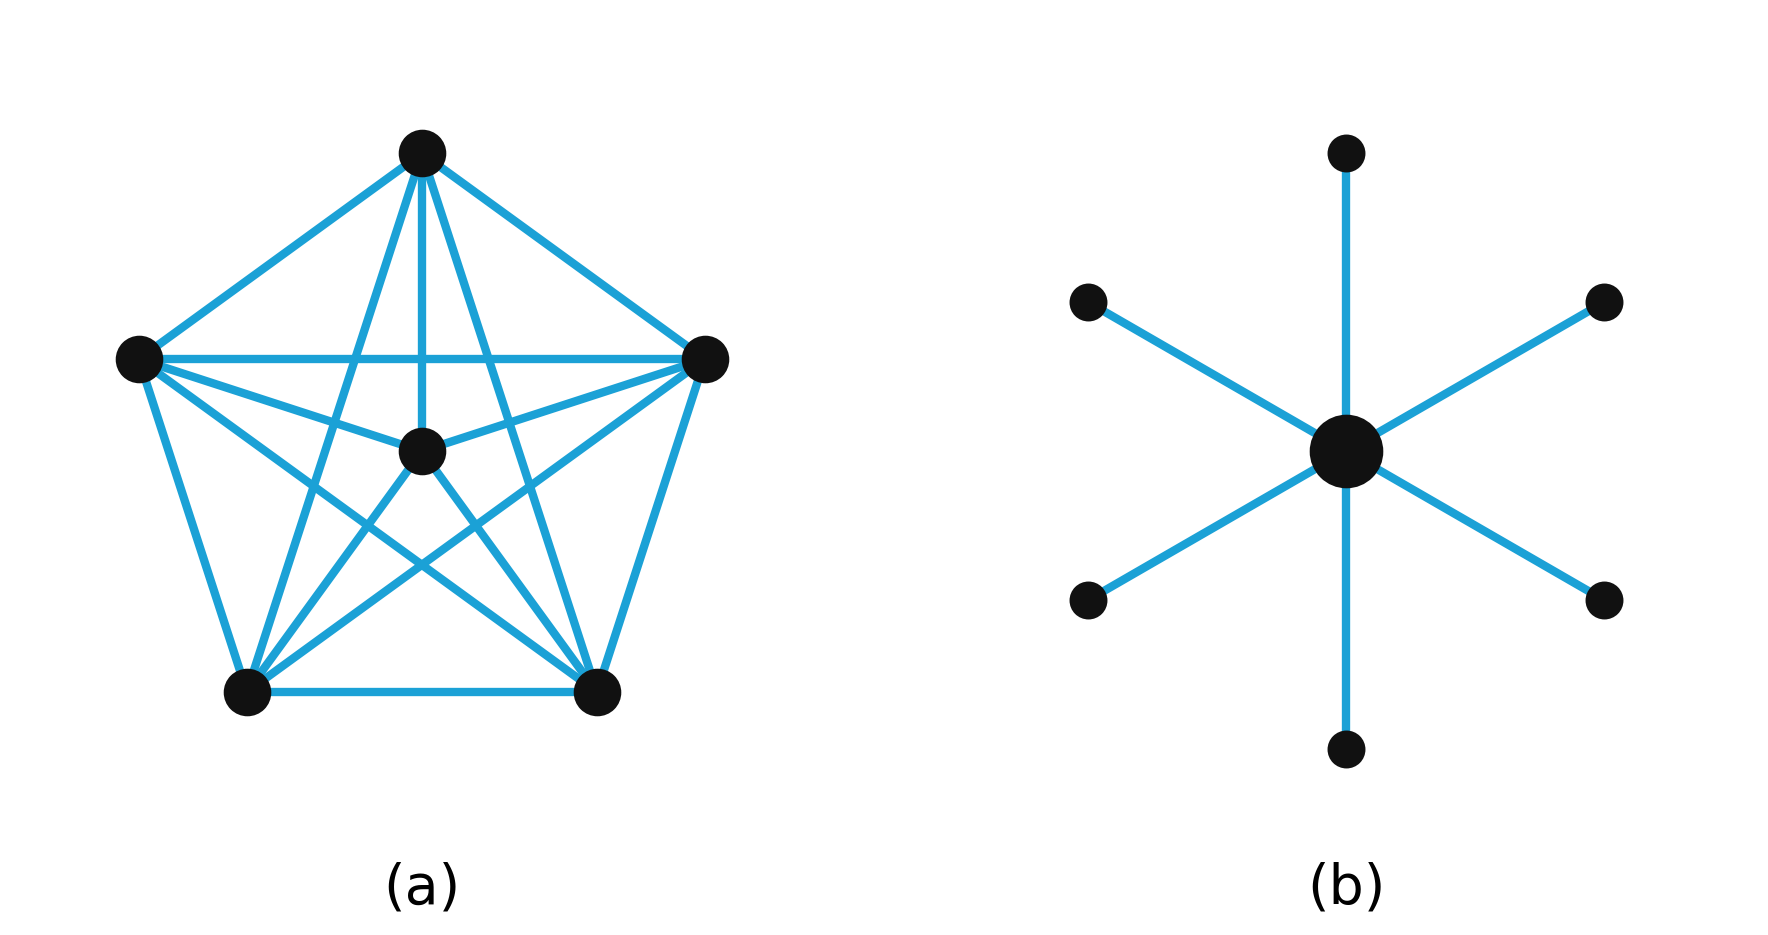
\includegraphics[width=0.5\linewidth]{images/hsvsp2p.png}
    \caption{Comparison of hub-and-spoke (HS) network and point to point (P2P) network structure. Source: \cite{AIFig8} \cite{HSvsP2P} }
    \label{fig:HSvsP2P}
\end{figure}

Hub and spoke networks are widely used across different industries including the logistics and freight distribution industry \cite[p.1]{CostHubSpoke}, the aviation industry \cite[p.1-2]{Aviation21} and cloud computing infrastructure \cite{Cloud}. In a traditional point to point transport (P2P) network (see a in \ref{fig:HSvsP2P}), goods (or passengers) are transported from dispatch location to the final destination. However, it may not be feasible in terms of cost to make these deliveries to the final destination. This is because shipping to multiple different final destinations requires dedicated trucks on each route by each dispatch location. This can result in cost loss caused by insufficient trucks with a full load being carried \cite[p.1]{CostHubSpoke}. An alternative to this P2P network is a hub and spoke (HS) (see b in Figure \ref{fig:HSvsP2P}) network where goods are collected at a central hub from which they are shipped to the final destinations which we call spokes \cite{HubSpoke}. This means that the goods can be collected from various dispatch points and shipped in bulk to their final destinations. This reduces the number of dedicated trips from each dispatch location. However, the hub's unloading capacity is finite and can therefore serve as a bottleneck when multiple trucks arrive simultaneously. Congestion and transport delays at the hub can have detrimental effects downstream on the logistics network resulting in an overload or possible failure of the hub \cite[p.2]{CostHubSpoke}. This is why trip scheduling is an important tactic to avoid such a scenario.

Trip scheduling has been looked at primarily through the lens of optimisation techniques such as cross entropy optimisation \cite{WadhawanTrain} which searches different permutations to minimise span of the schedule, i.e. the total time required to complete all trips. However, such optimisation techniques have not been studied in detail for this paper. We pay attention to combinatorial frameworks to tackle this area.

Juggling models provide a natural format to frame this problem by implementing combinatorics. Juggling states are able to encode the current and future arrivals of trucks to the hub with the passage of time. The same way a juggler schedules balls to land on future beats, trips are scheduled to arrive at the hub at future points in time. By treating these arrivals as random, the tools of juggling state graphs and Markov chains can be used to study the long-run behaviour of a hub-and-spoke network. 

Using this framework, we model a hub served by up-to three trucks and simulate its behaviour under varying numbers of unloading bays and varying travel times. Our experiments show that hub capacity and trip timing both have a marked economic impact. Increasing the number of bays from one to two improves profitability, but adding a third bay yields little benefit as it is rarely utilised. On the other hand increasing travel times reduces both revenue and cost as less number of trucks are unloaded over time. These results illustrate how juggling-based models can inform decisions about hub capacity and trip scheduling, although we note the model has not yet been calibrated against a real hub-spoke network.

\section{Background}

\begin{figure}[!htb]
    \centering
    \includegraphics[width=0.25\linewidth]{Screenshot 2026-08-04 at 3.47.55 PM.png}
    \caption{Hub and Spoke Transport Network with three spokes at varying distances. Sources: \cite{AIFig9} \cite{AIFig11}}
    \label{fig:hub-spoke-3}
\end{figure}

A basic hub-and-spoke transport network is displayed in Figure \ref{fig:hub-spoke-3}. Here, the central hub is the circle labelled Hub in purple at the centre of the figure. The spokes are ports located at varying distances from the hub labelled A till C. Trucks route their cargo through a central hub from their spokes. The benefit of utilising a hub-and-spoke model has been noted by \cite{Aviation21} in the context of the aviation industry where it serves to maximise profits. This is because airlines are able to carry a number of passengers with varying final destinations to the same central airport. 


However, as described by \cite{WadhawanTalk} for their train model which is similar to a hub-and-spoke network, the trains may have to queue up at the central port (Hub) when arriving from silos (spokes A-C) at the same time. This may be due to limited unloading capacities at the port. Juggling notation has been used to model this train system in \cite{WadhawanTalk}'s talk but they do not continue with this approach in depth in the related paper \cite{WadhawanTrain}. Instead, they focus on an optimisation method to construct their trip sequences. 


\subsection{Siteswap Notation and Juggling Models}
\begin{figure}[!htb]
    \centering
    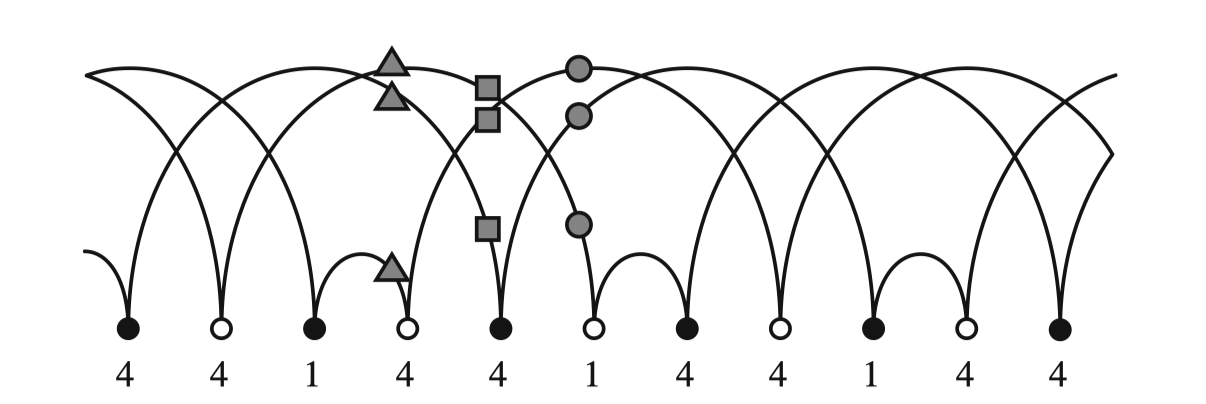
\includegraphics[width=0.5\linewidth]{images/image.png}
    \caption{Juggling diagram of juggling pattern 441. Source: \cite[p.46]{Polster2003}}
    \label{fig:jugg_diag2}
\end{figure}


In order to describe juggling models, a notation was developed by various mathematicians around the same time and has been described by \cite[p.5 -- 6]{Mays} in detail. It is known as siteswap notation. According to this notation, time is counted in the form of discrete beats. It is assumed that a juggler throws and catches balls for an infinite amount of time with no lag time between catching and throwing the ball. Therefore, catching and throwing can happen on the same beat. When the juggler throws this ball, it is associated with a certain non-negative integer $h$ which is called ``throw height''. As such, this h-throw lasts $h$ beats of time. This can be observed in figure \ref{fig:jugg_diag2} where each black and white circle represents a ball caught at a time beat. The numbers 4, 4 and 1 represent the smallest repeating pattern of throw heights whose length is called its period. For example, a ball thrown at a height of 4 is caught 4 beats later and the period of the simple juggling pattern 441 is 3. 


\begin{figure}[!htb]
    \centering
    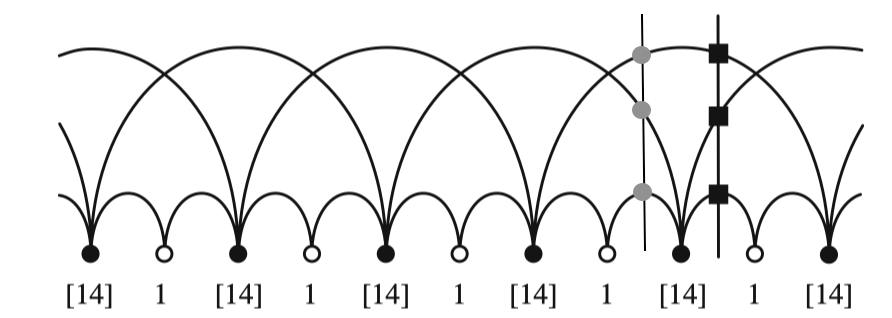
\includegraphics[width=0.5\linewidth]{images/multiplexjuggle.png}
    \caption{The juggling diagram of the multiplex juggling sequence [14]1. Source: \cite[p.66]{Polster2003}}
    \label{fig:multiplexjuggle}
\end{figure}

Juggling patterns are split into two classes: simple and ``multiplex''. In a simple pattern, at most one ball can be caught and thrown on any given beat \cite[p.8]{Polster2003}, whereas a multiplex pattern relaxes this restriction by allowing more than one ball to be caught and thrown simultaneously \cite[p.65]{Polster2003}. Both classes are characterised by two parameters: the number of balls being juggled, $b$, and the maximum throw height, $h$. A simple pattern such as 441 specifies a single throw height per beat. However, for a multiplex pattern, we use square brackets to group simultaneous throws on the same beat. Note that in figure \ref{fig:multiplexjuggle}, square brackets are used to show simultaneous throw height and the juggling pattern is [14]1. Reading from left to right, the first black round circle represents throwing 2 balls at a height of 1 and 4 respectively. The first white circle that follows represents a single ball thrown to a height of 1. This pattern repeats for the remaining figure.

\begin{figure}
    \centering
    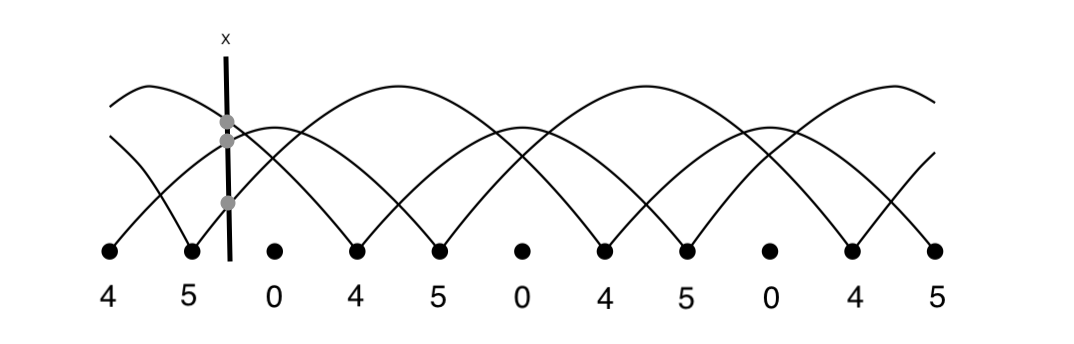
\includegraphics[width=0.5\linewidth]{images/add-drop.png}
    \caption{Juggling diagram of a juggling sequence 450 where a ball can be added or dropped. Source: \cite{Mays}}
    \label{fig:add-drop}
\end{figure}


Additionally, we will describe the ``add-drop'' model as mentioned in \cite[p.115]{Warrington2005}. In this model, a juggler can add additional balls to the pattern or drop existing ones. If the juggler faces a wait i.e. no ball landing at t=0 as can be seen after the vertical line in figure \ref{fig:add-drop}, the juggler can add an extra ball to the pattern at this beat. If they have a ball at t=0, they can choose to drop this ball as well. 

Hub-and-spoke models can be described using juggling models. Juggling describes the arrival of a sequence of balls in a juggler's hands in discretised time after they have been thrown to a certain height. This mirrors the arrival of trucks to a hub at hourly intervals. The trucks can be treated as balls whereas the arrival time of a truck can be treated as the height of the throw of a ball. For example, if a juggler throws a ball with a throw height of 3, the ball will land after 3 time beats. This is equivalent to a truck returning to the hub in three hours where each beat represents an hour. Lastly, multiplex juggling, the specific juggling model we focus on, allows for multiple balls to land in a juggler's hands at the same time. This is analogous to multiple trucks arriving simultaneously at a central hub.


\subsection{State Transitions}

Based on the notation described above, throw heights determine the beat at which the ball will land in the future. As described in \cite{Polster2003}, these landings can be represented as a pattern of 1's and 0's. Assuming that the juggler has been captured in a moment in time, represented by the three triangles in figure \ref{fig:jugg_diag2}. These balls (represented by the triangles) will land in the juggler's hands in successive beats one after the other. The landing state, which is also described as the juggling state, can be written as 11100. Here, each number is separated by a time beat where 1 represents a ball landing and 0 represents no balls landing. Since a ball can be thrown up to 5 beats into the future, extra 0's are included to account for those potential landing slots as shown in figure \ref{fig:bit-transitions}. The ball at t=0 is thrown to a height of 4 thereby reaching state 11010. Note that the remaining 1's and 0's between t=1 till t=4 shift  to the left by one time step to indicate that a beat has passed between the transition. The state transition described can be seen in figure \ref{fig:bit-transitions}. The intermediate step is omitted in later transition diagrams.
\begin{figure}[!htb]
    \centering
    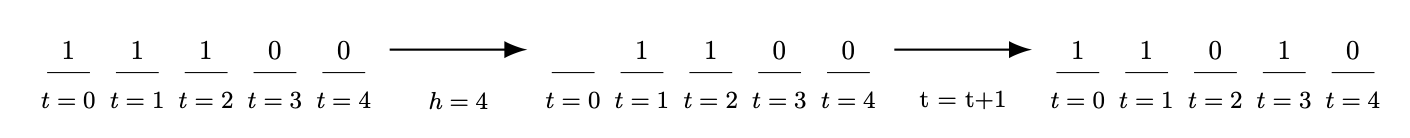
\includegraphics[width=1\linewidth]{images/state_trans.png}
    \caption{Transition between juggling states for a throw of height $h=4$. Source: \cite{AIFig12} \cite{AIFig15}}
    \label{fig:bit-transitions}
\end{figure}


However, different rules apply to simple and multiplex juggling states. In a simple juggling model, multiple balls cannot be caught (or thrown) at the same time. This means that two balls cannot arrive simultaneously in the future. However, multiplex juggling allows for this constraint to be lifted. Observe the vertical line that intersects the path of the three balls thrown by the juggler with grey circles in figure \ref{fig:multiplexjuggle}. We note the path of these three balls. The first ball lands at t=0, the second lands at t=0 and the third ball lands at t=2. This results in a juggling state 20100 where we assume a maximum throw height of 5. By throwing the balls at t=0 through a height of 1 and 4, we land at the state 11010. This representation can be seen in \ref{fig:multibit-transitions}

\begin{figure}[!htb]
        \centering
        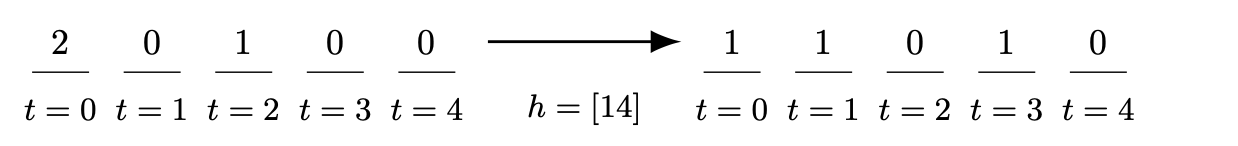
\includegraphics[width=0.75\linewidth]{images/multiplex_state.png}
        \caption{Diagram representing transitions between juggling states and their respective throw heights for a multiplex juggling system. Source: \cite{AIFig12}}
    \label{fig:multibit-transitions}
\end{figure}

\begin{figure}[!htb]
    \centering
    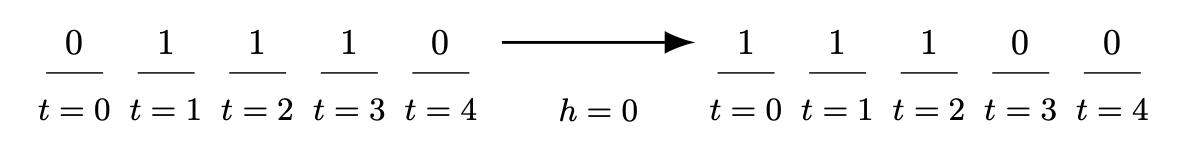
\includegraphics[width=0.75\linewidth]{images/zero_trans.png}
    \caption{Transition between juggling states where no ball is thrown or caught denoted by throw height of 0. Source: \cite{AIFig12}}
    \label{fig:zero-transitions}
\end{figure}

Additionally, if the juggler is faced with the situation of no balls arriving at the current time beat such as 01110, no action will be required by the juggler and such a throw is called a 0-throw. The sequence moves to the left resulting in the state 11100 as seen in figure \ref{fig:zero-transitions}. However, this is not the only 0-throw. Adding or dropping a ball is also considered a 0-throw. If a juggler has a ball at t=0, they can drop it and this can be seen by the dashed arrow in figure \ref{fig:drop-transitions}. If a juggler has no ball at t=0, an additional ball can be inserted anywhere in the sequence to increase the number of balls being juggled. This situation can be seen with the dotted arrow in figure \ref{fig:add-transitions}. Note that, in this system, addition and dropping of balls is treated by moving one time step forward after addition or removal of the balls. 

\begin{figure}[!htb]
      \centering
      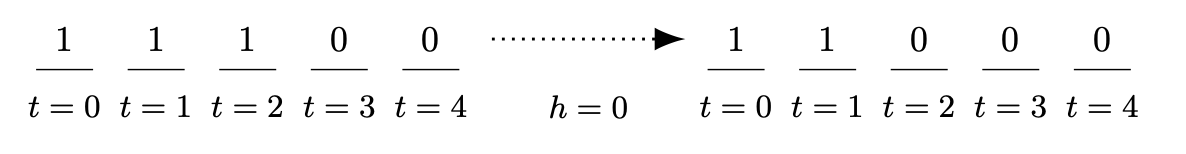
\includegraphics[width=0.75\linewidth]{images/dropped_ball_State.png}
      \caption{Transition between juggling states where a ball is dropped from the system. Source: \cite{AIFig12}}
    \label{fig:drop-transitions}
\end{figure}


\begin{figure}[!htb]
      \centering
      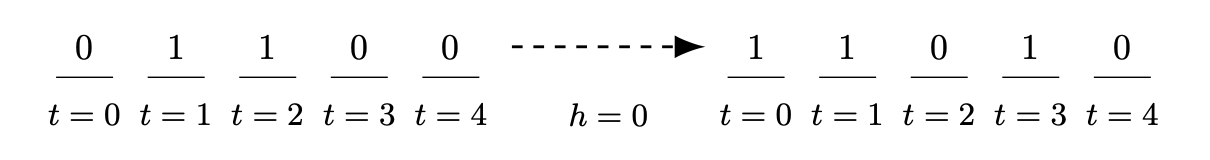
\includegraphics[width=0.75\linewidth]{images/add_ball_State.png}
      \caption{Transition between juggling states where a ball is added to the system. Source: \cite{AIFig12}}
    \label{fig:add-transitions}
\end{figure}



\subsection{Juggling State Graph}

\begin{figure}[!htb]
    \centering
    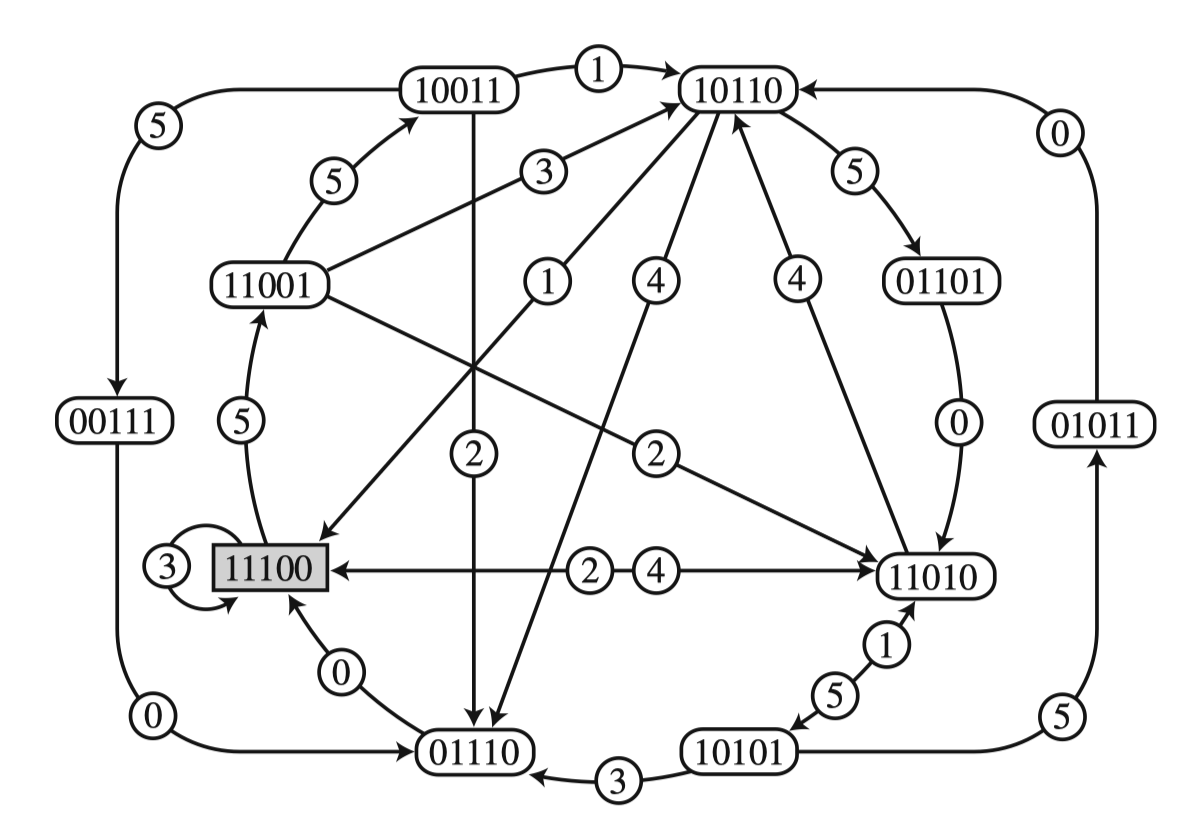
\includegraphics[width=0.5\linewidth]{images/state_graph.png}
    \caption{The simple 3 ball juggling state graph of height 5. Source: \cite[p.45]{Polster2003}}
    \label{fig:state_graph}
\end{figure}

By finding out the total states and the throw heights that connect them, we can create a graph known as a ``juggling state graph''. The graph for simple juggling  can be seen in figure \ref{fig:state_graph}. Here we note that to go from state 11001 to state 10011, we require a throw height of 5 whereas to reach state 11100 from state 01110, we must throw a 0 throw height. 

\subsection{Uniform Distribution \& Transition Matrix} \label{sec:unif_dist}
We note that a juggler has the ability to choose which state to transition into next based on the throw height. We assume that the juggler is equally likely to choose from $n$ allowed throw heights while in a given state $i$ in order to reach the next state $j$. Therefore, the juggler follows a uniform random process \cite[p.105]{ProbStatAlex} where the probability of transitioning from state $i$ to state $j$ is defined in equation \ref{eqn:pij}. We also assume that the future juggling state only depends on the current juggling state and permissible throw heights.


\begin{align}
        \label{eqn:pij} P_{ij} =\begin{cases}
                  \dfrac{1}{n} & \text{if state } j \text{ is reachable from state } i,\\[2mm]
                  0 & \text{otherwise}
              \end{cases}
    \end{align}

Juggling systems can be then be seen as stochastic processes where future juggling states are conditionally independent of their past given the present, that is they obey the Markov property as shown in equation \ref{eqn:markov_prop} \cite[p.1715]{MarkovChains}:
\begin{align}
    \label{eqn:markov_prop}P(X_{t+1} = x | X_1 = x_1, X_2 = x_2, ..., X_{t}=x_{t}) = P(X_{t+1} = x | X_{t}=x_{t})
\end{align}

According to \cite[p.1715]{MarkovChains}, when the probabilities of transitioning between states are independent of time, where time is measured in discretised steps, the probabilities can be collected into a square matrix $P$ known as the transition matrix, where each entry $Pij$ gives the probability of moving from state $i$ to state $j$ as seen in equation \ref{eqn:trans_mat}.

\begin{align}
    \label{eqn:trans_mat} P =
                        \begin{pmatrix}
                        P_{11} & P_{12} & P_{13} \\
                        P_{21} & P_{22} & P_{23} \\
                        P_{31} & P_{32} & P_{33}
                        \end{pmatrix}
\end{align}



\subsection{Stationary Distribution} \label{sec:st_dist}

\begin{theorem}[Perron-Frobenius Theorem {\cite[p.28]{PSAllNotes}}] 
\label{thm:perr} If a Markov chain is connected and aperiodic then 
\begin{itemize}
    \item There is a unique stationary distribution $\pi$
    \item For every initial vector p(0), we have 
    \begin{align}
        lim_{m \rightarrow \infty} p(0) P^m = \pi
    \end{align}  
\end{itemize}
    
\end{theorem}

Since the possible juggling states and possible transition probabilities between states are known, juggling state graphs can be encoded into a transition matrix $P$ in order to observe the long run behaviour of the juggling system. This approach has been taken by \cite[p.110]{Warrington2005} who had to calculate the stationary distribution vector $\vec{\pi}$ whose entries $\pi_i$ can be interpreted as the fraction of time spent by the Markov chain in the $i$th state. This interpretation of $\pi_i$ is valid when the stationary distribution exists and is unique. Since our finite Markov chain is connected and aperiodic as per definitions \ref{defn:connected} and \ref{defn:aperiodic}, theorem \ref{thm:perr} guarantees that the stationary distribution $\pi$ exists and is unique.

\begin{align}
    \label{eqn:st_eqn} (P^T - I)\vec{\pi}^T = 0   
\end{align}
where $I$ is the identity matrix. 


In order to calculate this stationary distribution, \cite{Warrington2005} finds the right eigenvector for $P^T$ corresponding to the eigenvalue 1 (for a definition of eigenvalue and eigenvectors refer here: \ref{sec:eigen}). The details of how to calculate this have been outlined in \cite[p.19--21]{PS2025Week12Lecture} and involves solving the homogeneous equation \ref{eqn:st_eqn}. We note that the solution is of the form $t\vec{v}$ where $t\in \Re$. This means that there are multiple solutions which are all scalar multiples of each other. In our case, the stationary distribution is a probability vector and therefore requires that $\sum{\pi_i} = 1$. Therefore, we normalise the solution obtained using equation \ref{eqn:norm_eqn} to find the stationary distribution vector.

\begin{align}
    \label{eqn:norm_eqn} \vec {\pi} = \frac{t\vec{v}}{t\sum v_i}
\end{align}

From here on, we will apply the multiplex juggling framework on the hub-and-spoke network defined above. Trucks travelling between hub and spokes will be modelled as balls, with their total travel time corresponding to the height of throws for the balls in the juggling system and time is counted in hourly beats. The resulting Markov chain will then be analysed to figure out the long run behaviour of the system. In context of the hub-and-spoke model, the stationary distribution of our Markov chain describes the fraction of time the network spends in each state of trucks in transit in the long run.


\section{Methods}

\subsection{Formulating the model and constructing the state graph}


In order to describe our model which utilises the juggling framework described in the sections above and applies it to the hub-and-spoke network, we gradually build up on as shown below.

\subsubsection{Multiplex juggling applied to hub-and-spoke network}
Assume that a company runs a hub-and-spoke model with three trucks. Depending on how far the spoke is from the hub, the travel times will vary. In this model, we assume that there are three spokes as seen in figure \ref{fig:hub-spoke-3} where the farthest spoke is three hours away. Time is counted in hourly increments (also known as beats). These trucks are constantly moving and delivering goods between the central hub and the three spokes. There is only one bay to unload trucks in a single beat. 
This means that if multiple trucks arrive at the hub simultaneously, only one truck can be unloaded on a single beat. 

We model this system using juggling sequences, where a truck's travel time back to the hub is represented as the height of a throw. If a truck departs from the hub and takes 3 hours to arrive back at the hub, it is considered a 3-throw. To explain this, we focus on an example. If we start with state 100, thrown to a height of 3, after one hour we would reach state 001 as shown in figure \ref{fig:juggling-states-graph} where the juggling states are created from the perspective of the hub. 

To understand how multiple trucks arriving simultaneously is dealt with, we look at another example. If two trucks arrive simultaneously, the corresponding state is 200 shown in figure \ref{fig:juggling-states-graph}. Since there is only one bay, one of these trucks would be thrown in to the future with a 1-throw to reflect that this is delayed and will be unloaded an hour later. Whereas, the other truck will be thrown to heights between 0 till 3. More specifically, starting with state 200, if two trucks are thrown with a throw height of 2 and 1 respectively, the throw heights would be represented as [21]. An hour later, the new state would be 110 as can be seen in figure \ref{fig:juggling-states-graph}. 

Lastly, it is assumed that the trucks can be thrown to any permissible height ranging from 0 till 3 to reach state $j$ given that they are in state $i$ and all throw heights are equally likely. Therefore, we can assume that a uniform probability distribution is followed. 

\subsubsection{Adding or removing trucks}
Trucks can be added or dropped from the system under certain conditions. In the real world, this would be equivalent to adding a truck to cater to additional routes to cater to increased demand or removing a truck because it has broken down or requires refuelling. 
% \RedComm{When would trucks be added or dropped if this was a model of a real system?}.
Trucks can be added at any time step if their addition does not exceed the maximum number of trucks allowed, which is three for our model, and they can only be added if there is no truck present at time t=0. Additionally, adding trucks is considered instantaneous that is time is not moved forward on addition of a truck to the system. The trucks can be dropped if there is at least 1 truck available at time t=0. Adding or dropping a truck is denoted by a throw height of 0. To differentiate these two in the juggling state graph we denote addition using a dotted arrow while a removal is denoted using a dashed arrow in the juggling state graph \ref{fig:juggling-states-graph}. 

\subsubsection{Varying the number of unloading bays}
To see the impact of unloading more than one truck in a single beat, we add in up to three bays. This allows us to unload two if there are two bays and three trucks if there are three bays simultaneously. We also assume that the maximum number of trucks that can be added or remove in a single beat depends on the number of bays. So if there are two bays, two trucks can be added or removed from the system in one time step. 


\subsubsection{Varying the throw height}
Lastly, we vary the throw height while keeping the number of cars limited to three to see the impact on simultaneous arrivals of trucks to the hub. The aim being that if the throw height is doubled, then it will take trucks longer to return to the hub. This would reduce the number of simultaneous arrivals to the hub.


\subsubsection{Final model}
Our final juggling model is denoted $J(\leq b,h, B)$. Here, b denotes the maximum number of trucks that our system can carry, h denotes the maximum throw height and B denotes the number of bays in the system. In particular, our primary model $J(\leq 3, 3, 1)$ has one bay. It's juggling state graph can be seen in figure \ref{fig:juggling-states-graph}. We will later vary the number of bays and throw heights to see their respective impacts on our system. 

We will now move on to finding out how to figure out the total number of valid states there are in this system given that there is only one unloading bay available.

\begin{figure}
    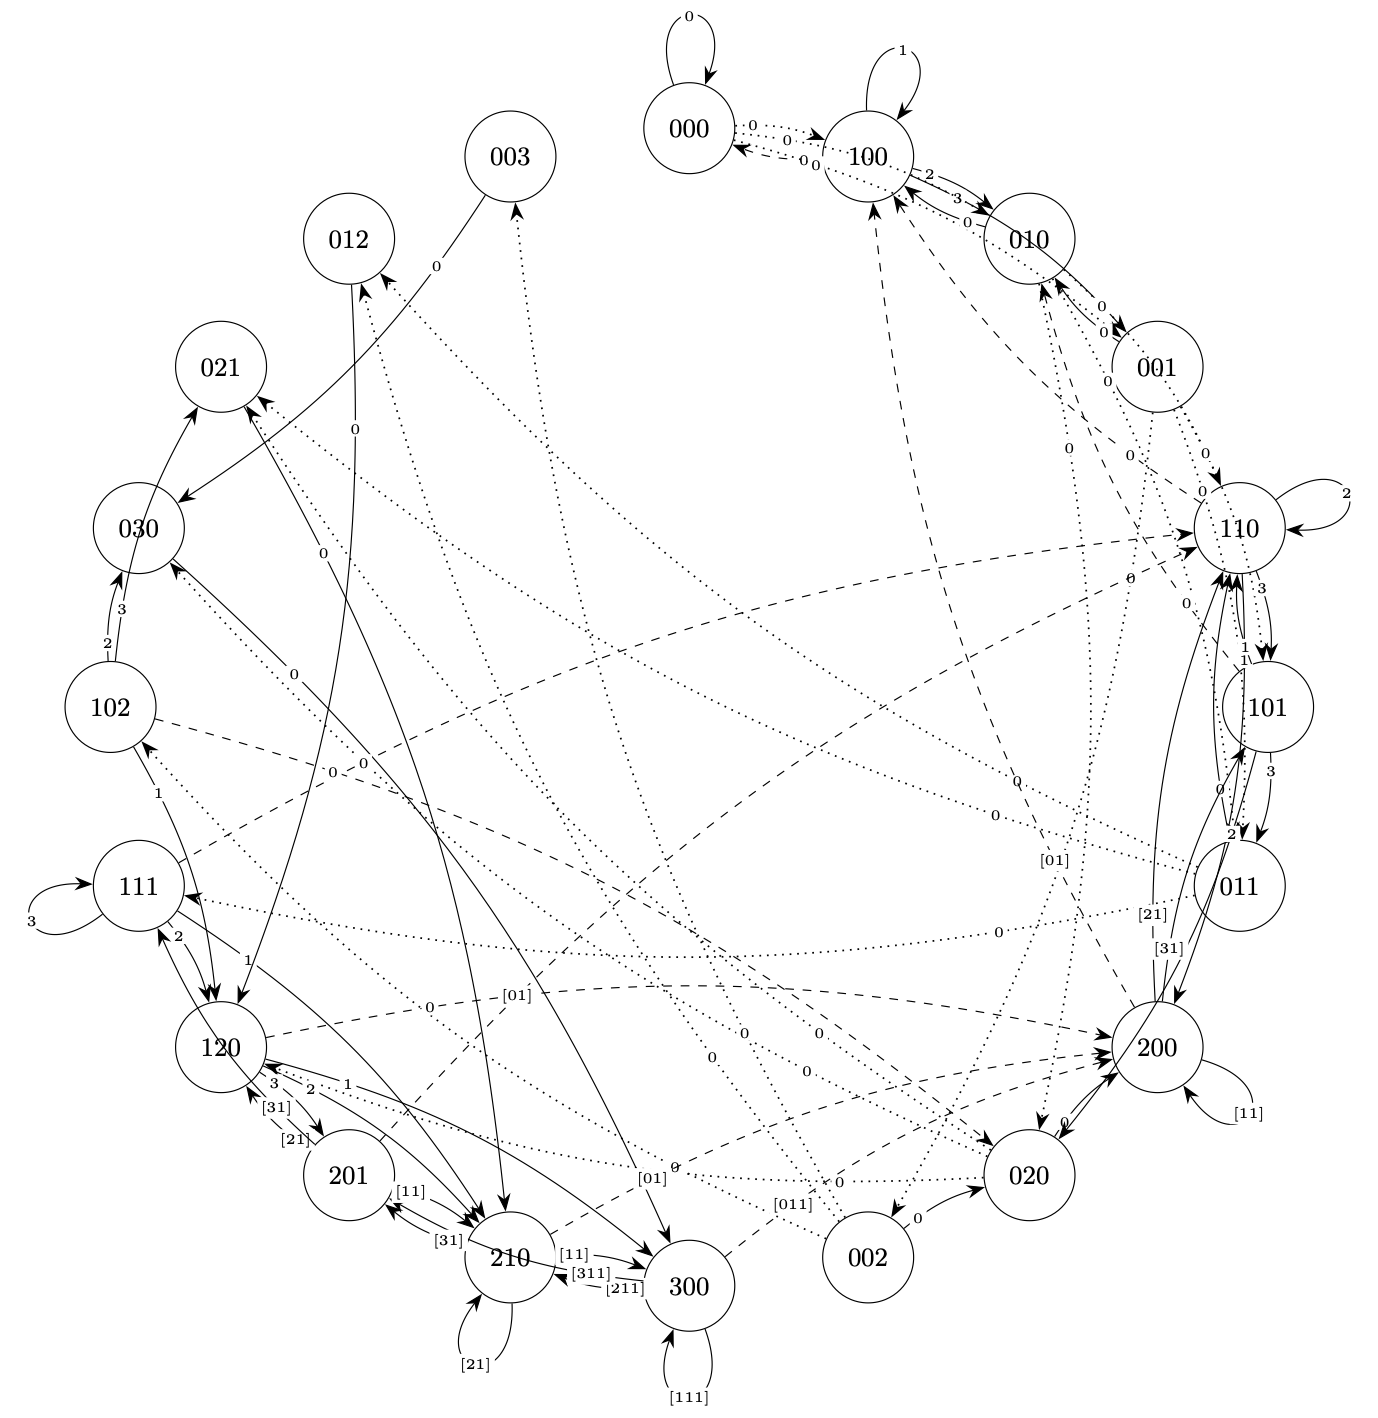
\includegraphics[width=1\linewidth]{images/state_graph_j331.png}
    \caption{Juggling state graph of up to 3 trucks that can travel for a maximum of 3 hours between the hub with 1 unloading bay and spoke for $J(\leq3, 3, 1)$. Source: \cite{AIFig10}}
  \label{fig:juggling-states-graph}
\end{figure}


\subsection{Number of states}
In order to find the number of states for a multiplex juggling system, we use the stars and bars method outlined in section \ref{sec:Number of states}. Since, the number of trucks in our system vary, we add up all the juggling states for the different number of balls. We are able to do so by using equation \ref{eqn:sum_starsbars} where $h$ is the maximum throw height, $b$ is the number of trucks and $b\_max$ is the maximum number of trucks allowed in our system. 

However, if we extend the number of trucks and height to values greater than 3, the equation changes. This is because of the limited  capacity to unload trucks at the unloading bays preventing certain throw heights leading to illegal states. Finding the equations for these specific cases extends beyond the scope of this paper. 

Our particular juggling system $J(\leq3, 3, 1)$ has been shown with all its states and transitions in the state graph in figure \ref{fig:juggling-states-graph}. Every edge carries a known probability as described in section \ref{sec:unif_dist}. This will let us treat the system as a Markov chain which we can then use to find the long run behaviour of the system. 

\subsection{Generating juggling states}
The algorithm used to generate the states and transitions of $J(\leq 3, 3, 1)$ is given in section \ref{sec:genmat} \footnote{Note that the lines of code are from the file \lstinline|CreateStMatrix_1Bay.m| unless stated otherwise}


This algorithm is adjusted slightly so that it can be used for the case where the bays are increased to two \footnote{The code for this can be found in the file \lstinline|CreateStMatrix_2Bay.m|} and three \footnote{The code for this can be found in the file \lstinline|CreateStMatrix_3Bay.m|}. The difference lies in how many balls can be added and how many balls can be thrown or dropped. If there are 2 bays, then upto two balls can be added and upto two balls can be thrown to specified heights rather than just being throw to height 1. Additionally if the throw height is doubled, the algorithm stays the same with the addition of initialising the throw height to double the value \footnote{The code for this can be found in the file \lstinline|CreateStMatrix_1Bay_6H.m|}.

\subsection{Encoding state graph as a transition matrix}

By using equation \ref{eqn:pij}, we encode the state graph for $J(\leq 3, 3, 1)$ in figure \ref{fig:juggling-states-graph} as a transition matrix \footnote{Note that the following lines of code are from the file \lstinline|SimRun_1Bay| unless stated otherwise} \footnote{The matrix can be found on lines 2 -- 21} shown in equation \ref{eqn:trans_matrix} where the probability of moving from state $i$ to state $j$ is assumed to follow a uniform random distribution. For example, by observing figure \ref{fig:juggling-states-graph}, we note that state 110 can either transition to state 100 by dropping a ball with a throw height of 0, state 110 with a throw height of 2, state 101 with a throw height of 3 or state 200 with a throw height of 1. It is assumed that each of these states can be reached with equal probability value of $1/4$ and correspond to the entries $P_{5,1}$, $P_{5,5}$, $P_{5,8}$ and $P_{5,10}$ \footnote{The row matrix containing these entries can be found on line 6} respectively. After applying this method to all states, the result can be seen in the transition matrix in \ref{eqn:trans_matrix}

By using this transition matrix, the stationary vector is found by finding the eigenvector associated with an eigenvalue of 1. This gives us the exact stationary distribution vector required. We also want to observe changes to the system over time by running a simulation.

\subsection{Convergence} \label{sec:conv}

To ensure that our simulation is behaving correctly, we must measure convergence of the simulation to the theoretical stationary distribution when run over a long period. To do so we calculate the residual sum of squares (RSSQ) \footnote{This calculation is done on line 93 } using equation \ref{eqn:rssq} which sums the squared differences between corresponding components of the simulated and theoretical stationary distributions.

\begin{align}
    \label{eqn:rssq} RSSQ = \sum_{i=1}^{i=20}{(\vec{\pi}_i - \vec{\hat{\pi}}_i)^2}
\end{align}

where $\vec{\pi}$ \footnote{This result and its calculation can be found on line 28 } is the theoretical stationary state vector and $\vec{\hat{\pi}}$ \footnote{This calculation can be found on line 92 } is the simulated stationary state vector at iteration $k$ where $k$ is between $1$ and $10^5$

RSSQ is calculated at each iteration and the final RSSQ value is found by averaging the values across all iterations.

\subsection{Addition of cost and revenue in the model}

In order to calculate the total cost and revenue collected from serving trucks at the hub we employ two equations to generate total revenue and total cost. The cost consists of three components as outlined in equation \ref{eqn:cost}; namely 
\begin{itemize}
    \item Fixed cost: is the cost associated with running the hub which includes paying the staff and the bills.
    \item Bay cost: is the cost of unloading a truck given a certain number of bays. If there is more than one unloading bay, the bay cost goes up to incorporate the cost of running this additional bay.
    \item Delay cost: is the cost incurred for delaying a car from being serviced. For example, if two trucks arrive at the hub but there is only one unloading bay to service them, then the other car gets delayed by an hour. This incurs a delay cost in the model.
\end{itemize}

On the other hand, we have revenue which consists of a single component known as the: 
\begin{itemize}
    \item Base revenue: this is the revenue generated by serving trucks at the unloading bay. The greater the number of trucks unloaded, the greater the revenue generated. 
\end{itemize}

\begin{align}
    \label{eqn:cost} TC_t = TC_{t-1} +  BC \times NP_t + DC \times NT_t  + FC
\end{align}

\begin{equation}
    \label{eqn:revenue}TR_t = TR_{t-1} + BR \times NT_t
\end{equation}

where, 
\begin{itemize}
    \item $t$ is the current time step in the iterations
    \item $TC_t$ is the total cost at time t 
    \item $BC$ is the bay cost of unloading one or two or three trucks
    \item $DC$ is the delay cost of one truck
    \item $FC$ is the fixed cost of operating the hub
    \item $NP_t$ is the number of trucks processed (unloaded) at time t
    \item $NT_t$ is the number of trucks delayed at time t
    \item $TR_t$ is the total revenue accumulated by time t
    \item $BR$ is the base revenue
\end{itemize}

\subsection{Running Simulation for $J(\leq 3,3,1)$} \label{sec:runsim}

\begin{algorithm}
In order to observe the changes to the system $J(\leq 3,3,1)$ over time, a simulation is run based on Markov Chain Monte Carlo simulation \cite[p.3]{MCMC}. 
% Here you describe the algorithm that you are going to implement
\begin{enumerate}
    \item Load the transition matrix $P$ from equation \ref{eqn:trans_matrix} where each row lists the transition probabilities from the current state $i$ to future state $j$ \footnote{This can be found on lines 2 -- 21 }
    \item Theoretical stationary distribution: Find the eigenvector and eigenvalues of transposed $P$ that is $P^T$ and normalise it \footnote{This calculation can be found on lines 27 -- 28 .}
    \item Initialise simulation parameters\footnote{These values can be found on lines 31 -- 33 }, economic constants \footnote{These values can be found on lines 36 -- 42 }, storage \footnote{These vectors can be found on lines 44 -- 45 } and vectors grouping the juggling states \footnote{These vectors can be found on lines 47 -- 49 }.
    \item For each seed and each starting state $k$ 
    \begin{enumerate}
        \item Initialise state vector \footnote{This vector can be found on line 59 }, where each position represents a state, to track the number of times a state is visited in $n$ iterations
        \item Loop over $n$ iterations \footnote{This loop begins at line 65}
        \begin{enumerate}
            \item Sample the next state from row $k$ of $P$ using inverse transform sampling \cite{InvTrans} \footnote{The calculation is done on lines 61 -- 75}. The details are mentioned in section \ref{sec:invtrans}
            \item Update total cost and total revenue using equations \ref{eqn:cost} and \ref{eqn:revenue}. \footnote{These calculations are done on lines 76 -- 87 }.
            \item Find the simulated stationary vector $\vec{\hat{\pi}}$ using  equation \ref{eqn:norm}\footnote{This calculation is done on line 92} 
        \end{enumerate}
        \begin{align}
            \label{eqn:norm} \vec{\hat{\pi}} = \frac{\vec{s}}{\sum_i \vec{s_i}}
        \end{align}  
        where s is \lstinline|s_vec| and record RSSQ \footnote{This calculation is done on line 93 } (equation \ref{eqn:rssq})
        \item Store the final simulated stationary vector after $n$ iterations for the $k$th \footnote{This result is stored on line 95 }.
    \end{enumerate}

    \item Compute average cost and average revenue as \lstinline|(total_cost/num_states)/seeds| \footnote{This calculation is done on line 102 } and \\
    \lstinline|(total_revenue/num_states)/seeds| \footnote{This calculation is done on line 103 }
    \item Average across all seeds and starting states: the simulated stationary distribution \footnote{This vector is stored on line 107 }) and the RSSQ values, then compute the overall RSSQ \footnote{This value is calculated on line 109 . The vector used to calculate this value is calculated on line 108 of the same file} from the mean distribution.
\end{enumerate}
\end{algorithm}

\subsection{Experimentation} \label{sec:exp}
The algorithm can be extended to different scenarios with a varying number of bays and throw heights to see which results in a more cost efficient run of the hub-and-spoke system. In particular, we set up four different scenarios listed in table \ref{tab:experiments}.

Our initial hub-and-spoke model operates with one unloading bay and a maximum throw height of 3. Since there is only one bay, we eventually run into a problem of multiple trucks arriving at the hub simultaneously. To serve multiple trucks at once, we increase the number of bays that serve the trucks in experiment two \footnote{The calculations for this experiment are found in the file \lstinline|SimRun_2Bay.m|} and three \footnote{The calculations for this experiment are found in the file \lstinline|SimRun_3Bay.m|}. Constructing and operating this additional bay increases the cost of serving each truck. This is indicated by the increased bay cost in experiment two and three compared to experiment one. Finally, we double the throw height in experiment four while keeping the number of bays constant to reduce the arrival of multiple trucks to the hub, thereby decreasing the total delay cost. By varying the number of bays and throw height in our system, we can see if the net profit (equation \ref{eqn:profit}) can be increased.

\begin{align}
    \label{eqn:profit} AP = AR - AC
\end{align}

Where,
\begin{itemize}
    \item AR is the average revenue and averaged across all seeds and different starting states.
    \item AC is the average cost averaged across all seeds and different starting states.
\end{itemize}

\section{Results}
\subsection{Convergence} 
% \RedComm{These should be subsections, not subsubsections}
\begin{figure}
    \centering
    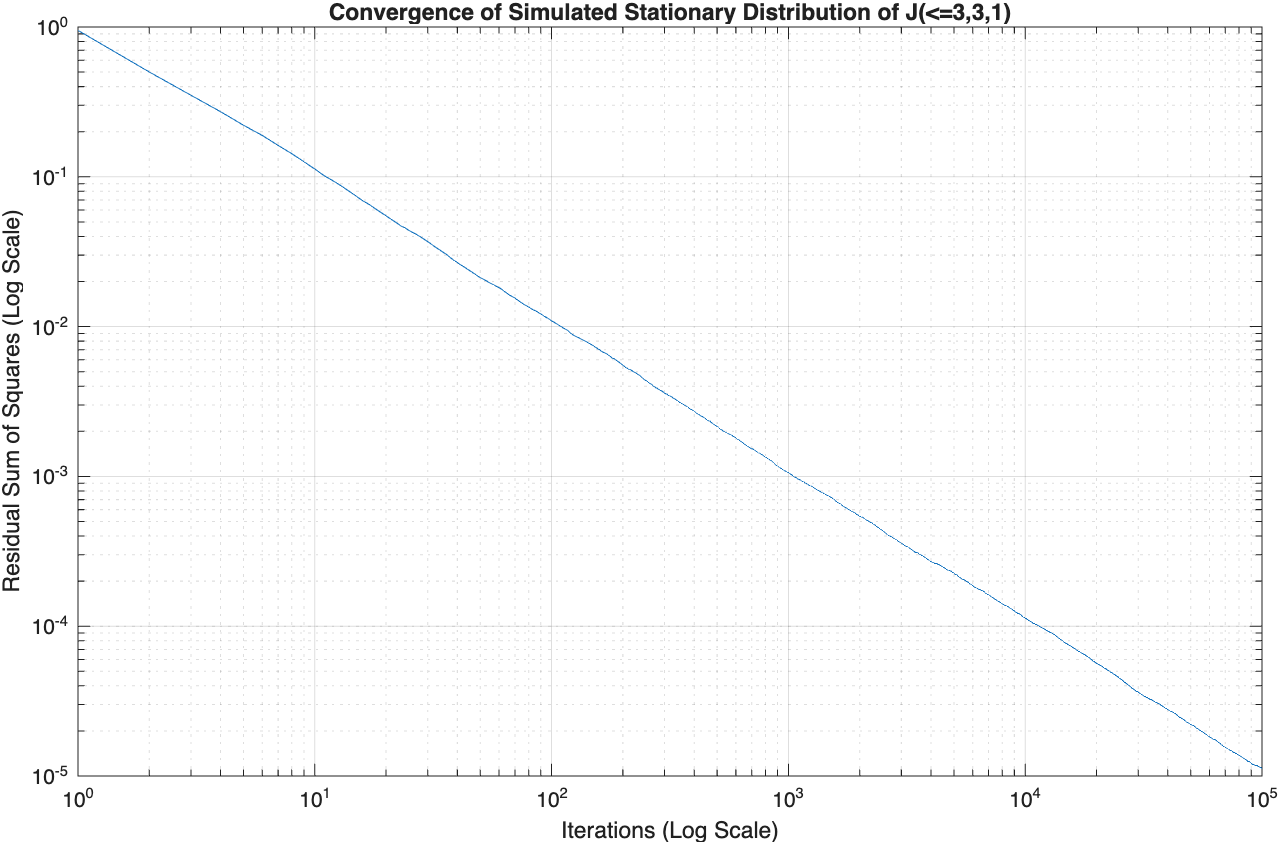
\includegraphics[width=1.0\linewidth]{images/logconvergence_1b3h.png}
    \caption{Residual sum of squares plotted against number of iterations to show convergence of simulated stationary distribution with theoretical stationary state for juggling system $J(\leq3,3,1)$ plotted on a log-log plot}
    \label{fig:logconvergence_1b3h}
\end{figure}


Figure \ref{fig:logconvergence_1b3h} \footnote{This graph has been plotted using the lines 135 -- 144 of the file \lstinline|SimRun_1Bay.m|} shows residual sum of squares (RSSQ) plotted against the number of iterations on a log-log plot for our juggling system $J(\leq3,3,1)$. The RSSQ values have been averaged over different starting states and different seeds. The simulation continues for $10^5$ \footnote{This value is stored on line 33 of the file \lstinline|SimRun_1Bay.m|} iterations and the RSSQ reduces over time in a linear fashion on the log-log scale.  The final mean RSSQ value at the end of the simulation is $3.37 \times 10^{-8}$ \footnote{This calculation can be found on line 109 of the file \lstinline|SimRun_1Bay.m|} as seen in figure \ref{fig:terminal_1b3h} \footnote{The calculations in this figure have been done using the lines 98 -- 111 of the file \lstinline|SimRun_1Bay.m|} which indicates that the simulated value gets closer to the theoretical value. Also note that the probability values for the theoretical stationary state and simulated stationary state distributions are nearly identical for all states as can be seen in figure \ref{fig:sim_1b3h}. This trend pertaining to a decreasing RSSQ value has been seen across the different experiments mentioned in section \ref{sec:exp}. The RSSQ log-log plots associated with these experiments can be found here: for experiment 2 refer to figure \ref{fig:logconvergence_2b3h} \footnote{This graph has been plotted using the lines 136 -- 145 of the file \lstinline|SimRun_2Bay.m|}, for experiment 3 refer to figure \ref{fig:logconvergence_3b3h} \footnote{This graph has been plotted using the lines 133 -- 142 of the file \lstinline|SimRun_2Bay.m|} and for experiment 4 refer to figure \ref{fig:logconvergence_1b6h} \footnote{This graph has been plotted using the lines 198 -- 207 of the file \lstinline|SimRun_1Bay_6H.m|}.

\subsection{Comparison of Simulated Stationary Distributions}



\begin{figure}
    \centering
    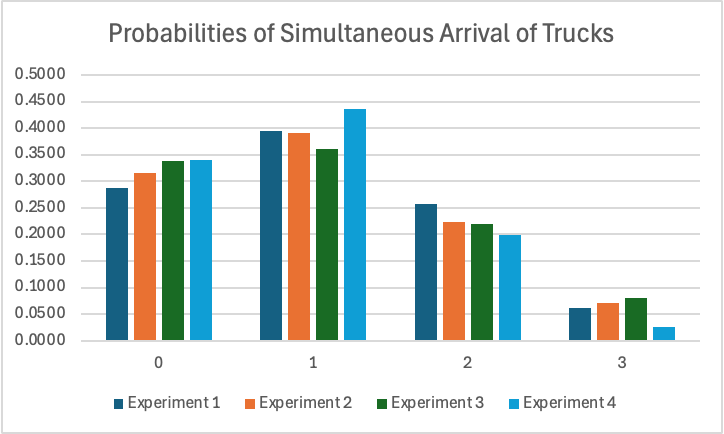
\includegraphics[width=1.0\linewidth]{images/states_probs_start_with.png}
    \caption{Probability of $k$ trucks arriving simultaneously at the hub for $k$ $\in \{0,1,2,3\}$, under each of the four experiments. The probabilities are calculated by summing the probabilities of each state starting with $k$ for each experiment. }
    \label{fig:states_probs_start_with}
\end{figure}


The simulated distribution results for the experiments described in section \ref{sec:exp} are displayed in figure \ref{fig:states_probs_start_with}. These probabilities indicate the fraction of time spent in each state where the states are grouped by the number of trucks arriving at the hub at t=0. We note that the probability of states starting with three is the lowest across all experiments. Further, the probability of states beginning with zero increase from experiments one till four with four having the highest probability. Similarly, the probability of states starting with two decreases across the experiments. Lastly, the probability of states beginning with three is the lowest in experiment four. The corresponding un-grouped probability results for experiments one till four can be found in the output images here: \ref{fig:terminal_1b3h}\footnote{This terminal has been produced using calculations on the lines 98 -- 118 of the file \lstinline|SimRun_1Bay|}, \ref{fig:terminal_2b3h}\footnote{This terminal has been produced using calculations on the lines 102 -- 121 of the file \lstinline|SimRun_2Bay|}, \ref{fig:terminal_3b3h}\footnote{This terminal has produced using calculations on the lines 99 -- 118 of the file \lstinline|SimRun_3Bay|} and \ref{fig:terminal_1b6h_ii}\footnote{This terminal has produced using calculations on the lines 179 -- 182 of the file \lstinline|SimRun_1Bay_6H|}.


\subsection{Economic results}

\begin{figure}
    \centering
    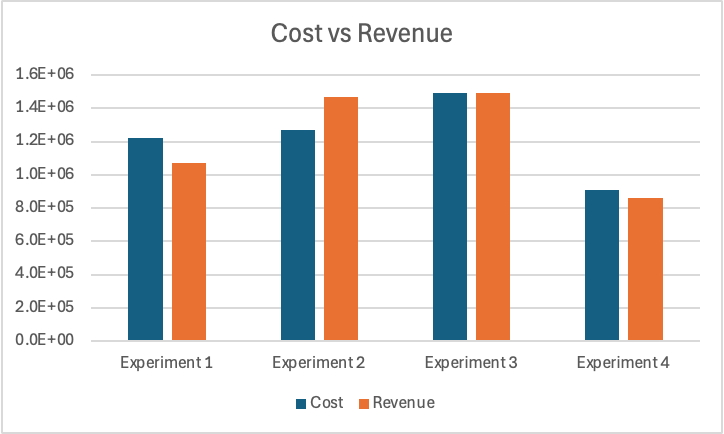
\includegraphics[width=0.75\linewidth]{images/cost_rev.png}
    \caption{Comparing the average revenue and average cost while varying the number of bays and throw heights. Source: Table \ref{tab:simrun}}
    \label{fig:cost_rev}
\end{figure}

\begin{figure}
    \centering
    
\includegraphics[width=0.75\linewidth]{profit.png}
    \caption{Plotting profit while varying the number of bays and throw heights. Source: Table \ref{tab:simrun}}
    \label{fig:profit}
\end{figure}

Figure \ref{fig:cost_rev} shows the revenue generated in orange and the cost incurred in dark blue from running the various experiments. Note that the highest cost and highest revenue is generated from experiment three whereas the lowest cost and lowest revenue is generated from experiment four. Figure \ref{fig:profit} shows the profit (or loss) incurred from the experiments. Note that the highest profit was approximately $0.20$ million which was generated from experiment two. Whereas the highest loss incurred was from experiment one with a value of approximately $0.16$ million.

\section{Discussion}
\subsection{Convergence}
The RSSQ values approaches zero showing that the simulation methodology has been correctly implemented. Further note that the plots pertaining to experiments one (\ref{fig:sim_1b3h}), two (\ref{fig:sim_2b3h}), three (\ref{fig:sim_3b3h})  and four (\ref{fig:sim_1b6h}) show that in all instances, the simulated stationary state probabilities closely match up with the theoretical stationary state probabilities.



\subsection{Economic analysis}

Note that experiment one where only one bay operates has a high cost with low revenue associated with it as seen in figure \ref{fig:cost_rev}. This results in the largest loss incurred out of all experiments as seen in figure \ref{fig:profit}. We believe that this is because the number of states with two trucks arriving simultaneously is high when compared to other experiments as can be seen in figure \ref{fig:states_probs_start_with}. This contributes to a higher total delay cost. We address this using two different approaches as follows:

\subsubsection{Increasing the number of bays}
In experiment two and experiment three, we increase the number of bays to two and three respectively. This results in a greater revenue in both scenarios compared to experiment one as seen in figure \ref{fig:cost_rev}. However, experiment two results in a higher profit compared to experiment three as shown in figure \ref{fig:profit}. We believe this is because in both experiments, the system does not spend a significant proportion of time in states where three cars arrive simultaneously at the hub as seen in figure \ref{fig:states_probs_start_with}. This leaves the third bay largely unutilised but the additional cost of the third bay in experiment three is still included in the bay cost for all trucks. This means that the total revenue generated has not significantly increased when compared to experiment two but the total cost does increase greatly as can be seen in figure \ref{fig:cost_rev}.

\subsubsection{Increasing the throw height}

In experiment four, we keep the number of bays constant and double the throw height. From figure \ref{fig:profit}, we note a lower loss when compared to experiment one. However, both the revenue and the cost as seen in figure \ref{fig:cost_rev} is lower when compared to experiment one. This could be because the system may be spending more time in states where no truck arrives that is states starting with zero as seen in figure \ref{fig:states_probs_start_with}. Since there is a fixed cost associated with operating the hub, the cost remains high and no revenue is generated when no trucks arrive at the hub.


\subsection{Limitations}
The primary limitation of this paper is that the model has not been calibrated or validated against any real hub-and-spoke system. We have no evidence that a true network operates as this model does, and significant further work would be required before any real-world recommendations could follow. For now it serves only as a tool for examining how throw height and the number of bays affect the economics of the system, not as a description of any physical network.

Two structural simplifications widen the gap to a real system. First, the model contains only three trucks and at most three bays, chosen so that every state and transition could be enumerated explicitly; this is far below the traffic an operational hub would face. Second, the assumption that trucks arrive under a uniform random distribution is unlikely to hold in practice, since trucks are dispatched by deliberate scheduling decisions rather than sent at random.



\subsection{Future work}
Future work would involve addressing the limitations mentioned above with the eventual aim of producing actionable recommendations for operating a hub-and-spoke system. The most important step would be to test the model at a larger scale with increased number of trucks and longer travel times. Secondly, the modelling assumptions would be relaxed; replacing the uniform distribution with a distribution that can better suit scheduled dispatching and actual costs associated with delaying and installing additional bays. The main aim of this calibration would be to closely align the model against a real world system and then use the cost and revenue equations mentioned in the paper to recommend an optimal number of bays and throw height for the real world system.

\subsection{Conclusion}

This paper used a Markov chain to model the arrival of trucks to a hub-and-spoke system and used its stationary distribution to analyse the behaviour of the system in the long run. The aim of the paper was to maximise the average profit generated by adjusting the number of bays and throw height. We found that increasing the number of bays improved the profit generated up to a point: a second bay substantially reduced delay costs, but a third produced little further gain because simultaneous arrivals of three or more trucks were infrequent. On the other hand, doubling the throw height reduced the frequency of simultaneous arrivals but not enough to make the single-bay configuration profitable, as the fixed costs incurred during the added idle time outweighed the delay savings. These findings hold within a small model and cannot necessarily be generalised to a larger model.


\section{Acknowledgements}
\begin{itemize}
\item I acknowledge that some of this template was adapted from an old University of Adelaide
Latex report template.
\item Help was provided by an AI agent (Claude.ai) to construct images, create aspects of the code mentioned in section \ref{sec:genmat} and help with sentence construction.
\begin{itemize}
    \item I acknowledge using my friend's (Shekhar's) AI agent (Claude) subscription. 
    % \RedComm{Good idea to acknowledge your funding source.}
\end{itemize}
\item Help was provided by my supervisor to develop the ideas of mapping hub-and-spoke systems to multiplex juggling.
\item Please find the github link here: \url{https://github.com/uzair-shah/MDSresearch_FinalReport_Bukhari_Syed}
\end{itemize}

\begin{thebibliography}{99}

\bibitem{HubSpoke}
Hapag-Lloyd AG. (2024, November 6). The Hub \& Spoke System in Shipping and Logistics Explained. \url{Hapag-Lloyd.com}; Hapag-Lloyd AG. \url{https://www.hapag-lloyd.com/en/online-business/digital-insights-dock/insights/2024/10/understanding-the-hub-spoke-system-in-container-shipping-.html}
\bibitem{Cloud}
Moreno, J., Palacios, A., \& Torkar, A. (2025). Hub-spoke network topology in Azure - Azure Architecture Center. In {Microsoft.com}. \url{https://learn.microsoft.com/en-us/azure/architecture/networking/architecture/hub-spoke}

\bibitem{Mays} Mays, A. (2006). \textit{Combinatorial aspects of juggling} [Honours Thesis, University of Melbourne]. \url{https://researchers.ms.unimelb.edu.au/~awmays@unimelb/Mays\_Juggling\_Thesis.pdf}

\bibitem{Warrington2005}
Warrington, G. S. (2005). Juggling Probabilities. The American Mathematical Monthly, 112(2), 105–118. https://doi.org/10.2307/30037409

\bibitem{Polster2003}
Polster, B. M. (2003). The Mathematics of Juggling. (1 ed.) Springer-Verlag London Ltd.

\bibitem{WadhawanTalk}
Wadhawan, I. B., Pudney, P., Howlett, P., \& Piantadosi, J. (2010). \textit{Juggling Trains}. [Slides]. University of South Australia. \url{https://uao365-my.sharepoint.com/:b:/r/personal/a1231659_adelaide_edu_au/Documents/AAStuff/Lecturing/MDSProjects/Juggling_2026/AllPapers/Wadhawan2010_JugglingTrains.pdf?csf=1&web=1&e=SQ7TID}

\bibitem{WadhawanTrain}
Wadhawan, I. B., Pudney, P., Howlett, P., \& Piantadosi, J. (2010). Scheduling trains with cross entropy optimisation. \textit{ANZIAM Journal, 51}, 332. \url{https://doi.org/10.21914/anziamj.v51i0.2594}

\bibitem{Invariance}
Math Is Fun. (2025). Invariant (Illustrated Math Dictionary). Math Is Fun. https://www.mathsisfun.com/definitions/invariant.html

\bibitem{PS2025Week12Lecture}
Mays, A. (2025). Week 12 Lecture [Lecture Slides]. Adelaide University MyLearning. \url{https://uao365-my.sharepoint.com/:b:/r/personal/a1231659\_adelaide\_edu_au/Documents/AAStuff/Lecturing/MDSProjects/Juggling\_2026/MDS2026\_Juggling\_Shared/PS\_2025\_Week12Lecture.pdf?csf=1&web=1&e=JfU6qC}

\bibitem{PSAllNotes}
Tuke, J. (2020). Chapter 1: Probability and statistics 2 [Lecture Notes]. Adelaide University MyLearning. \url{https://uao365-my.sharepoint.com/:b:/r/personal/a1947793_adelaide_edu_au/Documents/JugglingProject_Bukhari_SyedUzairShah_a1947793/Books%20and%20Papers/PS_AllNotes.pdf?csf=1&web=1&e=tR0cHB}

\url{https://uao365-my.sharepoint.com/:b:/r/personal/a1947793_adelaide_edu_au/Documents/JugglingProject_Bukhari_SyedUzairShah_a1947793/Books%20and%20Papers/PS_AllNotes.pdf?csf=1&web=1&e=oe8EXv}

\bibitem{MarkovChains}
Seabrook, E., \& Wiskott, L. (2023). A Tutorial on the Spectral Theory of Markov Chains. Neural Computation, 35(11), 1713–1796. \url{https://doi.org/10.1162/neco_a_01611}

\bibitem{MCMC}
Roughgarden, T., \& Valiant, G. (2023). CS168: The Modern Algorithmic Toolbox Lecture \#14: Markov Chain Monte Carlo. \url{https://web.stanford.edu/class/cs168/l/l14.pdf}


\bibitem{CostHubSpoke}
Xu, W., Huang, J., \& Qiu, Y. (2021). Study on the Optimization of Hub-and-Spoke Logistics Network regarding Traffic Congestion. Journal of Advanced Transportation, 2021(1), 1–16. \url{https://doi.org/10.1155/2021/8711964}

\bibitem{Aviation21}
Pels, E. (2020). Optimality of the hub-spoke system: A review of the literature, and directions for future research. Transport Policy, 104, A1–A10. \url{https://doi.org/10.1016/j.tranpol.2020.08.002}


\bibitem{HSvsP2P}
Cmglee. (2025). File:Comparison of point to point vs hub and spoke.svg - Wikimedia Commons. In Wikimedia.org. \url{https://commons.wikimedia.org/wiki/file:comparison_of_point_to_point_vs_hub_and_spoke.svg}

\bibitem{AIFig5}
Anthropic. (2026, May 2nd). Matrix to juggling state graph conversion [Generative AI chat]. Claude. \url{https://claude.ai/share/f822933f-0a0d-4bf8-bc88-909f48ba598c}

\bibitem{AIFig7}
Anthropic. (2026, May 2nd). Hub and spoke transport network diagram [Generative AI chat]. Claude. \url{https://claude.ai/share/13601884-47d7-4f67-8c6a-87b439c66cbc}

\bibitem{AIFig8}
Anthropic. (2026, July 11th). Side by side image comparison. [Generative AI chat]. Claude. \url{https://claude.ai/share/19ab5fad-5a5b-4420-a59a-9b17127331c3}

\bibitem{AIFig9}
Anthropic. (2026, July 11th). Three-truck hub and spoke distribution network. [Generative AI chat]. Claude. \url{https://claude.ai/share/cf79a5fa-9cdc-45ff-ad36-68dc71ed997a}

\bibitem{AIFig10}
Anthropic. (2026, July 20th). Three-truck hub and spoke distribution network. [Generative AI chat]. Claude. \url{https://claude.ai/share/b1a1aee1-e794-4766-9ef8-6014a781fb0d}

\bibitem{AIFig11}
Anthropic. (2026, July 21st). Hub and spoke network diagram in TikZ. [Generative AI chat]. Claude. \url{https://claude.ai/share/fb9187d9-62e7-4eb3-929e-6503a7750130}

\bibitem{AIFig12}
Anthropic. (2026, July 21st). Binary sequence diagram with Hamming distances. [Generative AI chat]. Claude.\url{https://claude.ai/share/c5ca28ca-9881-461b-ae1e-03fb42434cbf}

\bibitem{AIFig14}
Anthropic. (2026, July 22nd). String configuration with TikZ diagrams. [Generative AI chat]. Claude. \url{https://claude.ai/share/fa02ce3c-47c5-4923-a905-f9426a7b07a9}

\bibitem{AIFig15}
Anthropic. (2026, August 3rd). Clarifying intermediate steps in diagrams. [Generative AI chat]. Claude. \url{https://claude.ai/share/fb5b810e-6e37-4331-a55f-0b58108a99fe}

\bibitem{CountingStatesExample}
Anthropic. (2026, June 21st). TikZ diagram with dashes and filled circles. [Generative AI chat]. Claude. \url{https://claude.ai/share/3f648ad4-eacd-420c-96ab-4918934b9aa1}

\bibitem{WikiStarsBars}
Wikipedia Contributors. (2023). Stars and bars (combinatorics). In Wikipedia. \url{https://en.wikipedia.org/wiki/Stars_and_bars_(combinatorics)}

\bibitem{HockeyStick}
Wolfram Mathworld. (n.d.). Christmas Stocking Theorem. Wolfram Mathworld; https://mathworld.wolfram.com/ChristmasStockingTheorem.html.

\bibitem{ProbStatAlex}
Tsun, A. (n.d.). Probability \& statistics with applications to computing. Retrieved July 23, 2026, from \url{https://www.alextsun.com/files/Prob_Stat_for_CS_Book.pdf}

\bibitem{Rand}
The MathWorks, Inc. (2022). Matrix of Random Numbers. Mathworks.com. \url{https://www.mathworks.com/help/matlab/ref/double.rand.html}

\bibitem{CumSum}
The MathWorks, Inc. (2024). Cumulative Sum of Vector. Mathworks.com. \url{https://www.mathworks.com/help/matlab/ref/double.cumsum.html}

\bibitem{NormFunc}
The MathWorks, Inc. (n.d.). Vector and matrix norms - MATLAB norm. Www.mathworks.com. \url{https://www.mathworks.com/help/matlab/ref/norm.html}

\bibitem{CDFDefn}
Pishro-Nik, H. (2020). Cumulative Distribution Function. Probabilitycourse.com. \url{https://www.probabilitycourse.com/chapter3/3_2_1_cdf.php}

\bibitem{InvTrans}
Wikipedia. (2023). Inverse transform sampling. In Wikipedia. \url{https://en.wikipedia.org/wiki/Inverse_transform_sampling}


\end{thebibliography}


\newpage

\begin{center}
    {\LARGE \textbf{Appendices}}
\end{center}

\appendix

\section{Appendix}

\subsection{Eigenvectors and eigenvalues} \label{sec:eig}
In order to understand how a stationary distribution is calculated theoretically, we must first define what an eigenvector and eigenvalue is. As per \cite[p.1723]{MarkovChains}, an eigenvector of a matrix $P$ is a vector that is only multiplied by some number $\lambda$ when it is multipled by $P$. These vectors could be row vectors as in equation \ref{eqn:rowvec}


\begin{align}
    \label{eqn:rowvec} \pi^TP = \lambda \pi^T
\end{align}

in which case they are called left eigenvectors or they could be column vectors as in equation \ref{eqn:colvec}

\begin{align}
    \label{eqn:colvec} P\pi = \lambda \pi
\end{align}

in which case they would be called right eigenvectors. In both cases, the number $\lambda$ is called the eigenvalue of its respective eigenvector.

\subsection{Number of states}\label{sec:Number of states}

As per \cite[p.77]{Polster2003}, to find the total number of states for a multiplex juggling system, we can use equation \ref{eqn:stars_bars}. 
\begin{align}
    \label{eqn:stars_bars} state\_count = \binom{b+h-1}{b}
\end{align}

where $b$ is the number of balls and $h$ is the maximum throw height in the system. The method used to come to this formula is known as the stars and bars method and has been explained in \cite[p.12--13]{PSAllNotes}. We use a short example with 2 balls and a maximum throw height of three to explain this method. Since the throw height is three, we can visualise three time steps separated by vertical lines as shown below. 

\begin{figure}[!htb]
        \centering
        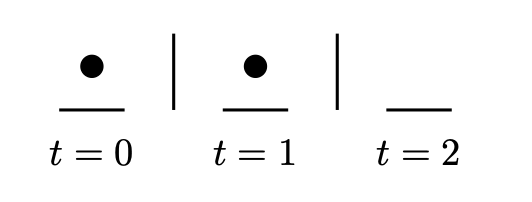
\includegraphics[width=0.25\linewidth]{images/counting_states.png}
        \caption{Diagram for representing two balls thrown to a maximum height of 3 at three beats. Source: \cite{CountingStatesExample}}
    \label{fig:state_count}
    \end{figure}
If we represent the balls as stars, then we have two balls which we can place on any time step, which are separated by bars. This results in six distinct cases laid out in in figure \ref{fig:starsbars}. By using \eqref{fig:starsbars}, we can find the toal number of ways to do it as shown in equation \eqref{eqn:count_starsbars}.


\begin{figure}
      \centering
      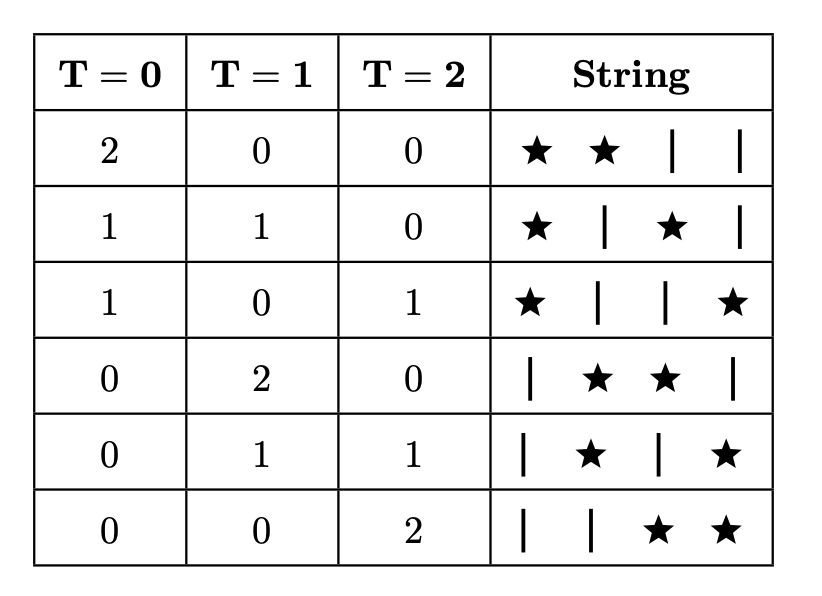
\includegraphics[width=0.5\linewidth]{images/table_stars.png}
      \caption{Six configurations of two balls in three time slots and their stars and bars representations. Sources: \cite{WikiStarsBars} \cite{AIFig14}}
  \label{fig:starsbars}
  \end{figure}

\begin{align}
    \label{eqn:count_starsbars} state\_count = \binom{2 + 3 - 1}{2} = 6
\end{align}

If we allow the case where balls can be added or discarded from the system, we can extend equation \ref{eqn:stars_bars} by including a summation symbol to calculate all possible juggling states for the multiplex system with a varying number of balls from 0 balls all the way to $b\_max$ balls where $b\_max$ is the maximum number of balls allowed to be added in to the system as seen in equation \ref{eqn:sum_starsbars}

\begin{align}
    \label{eqn:sum_starsbars} total\_states\_count = \sum_{b=0}^{b\_max}\binom{b + h - 1}{b}
\end{align}

\subsection{Transition Matrix}
Transition matrix pertaining to our initial model has been written down below and has been referenced in section 4.4.
\begin{align}
    \label{eqn:trans_matrix}
    P = \frac{1}{4}
    \begin{bmatrix}
    1 & 1 & 1 & 1 & 0 & 0 & 0 & 0 & 0 & 0 & 0 & 0 & 0 & 0 & 0 & 0 & 0 & 0 & 0 & 0 \\
    1 & 1 & 1 & 1 & 0 & 0 & 0 & 0 & 0 & 0 & 0 & 0 & 0 & 0 & 0 & 0 & 0 & 0 & 0 & 0 \\
    1 & 0 & 0 & 0 & 1 & 1 & 1 & 0 & 0 & 0 & 0 & 0 & 0 & 0 & 0 & 0 & 0 & 0 & 0 & 0 \\
    0 & 0 & 1 & 0 & 0 & 0 & 1 & 1 & 1 & 0 & 0 & 0 & 0 & 0 & 0 & 0 & 0 & 0 & 0 & 0 \\
    1 & 0 & 0 & 0 & 1 & 0 & 0 & 1 & 0 & 1 & 0 & 0 & 0 & 0 & 0 & 0 & 0 & 0 & 0 & 0 \\
    0 & 0 & 0 & 0 & 0 & 0 & 0 & 0 & 0 & 1 & 1 & 1 & 1 & 0 & 0 & 0 & 0 & 0 & 0 & 0 \\
    0 & 0 & 0 & 0 & 1 & 0 & 0 & 0 & 0 & 0 & 0 & 0 & 1 & 1 & 1 & 0 & 0 & 0 & 0 & 0 \\
    0 & 0 & 1 & 0 & 1 & 1 & 1 & 0 & 0 & 0 & 0 & 0 & 0 & 0 & 0 & 0 & 0 & 0 & 0 & 0 \\
    0 & 0 & 0 & 0 & 0 & 1 & 0 & 0 & 0 & 0 & 0 & 0 & 0 & 0 & 1 & 1 & 1 & 0 & 0 & 0 \\
    1 & 0 & 0 & 0 & 1 & 0 & 0 & 1 & 0 & 1 & 0 & 0 & 0 & 0 & 0 & 0 & 0 & 0 & 0 & 0 \\
    0 & 0 & 0 & 0 & 0 & 0 & 0 & 0 & 0 & 1 & 0 & 0 & 0 & 0 & 0 & 0 & 0 & 1 & 1 & 1 \\
    0 & 0 & 0 & 0 & 0 & 0 & 0 & 0 & 0 & 0 & 0 & 0 & 0 & 0 & 0 & 0 & 0 & 4 & 0 & 0 \\
    0 & 0 & 0 & 0 & 0 & 0 & 0 & 0 & 0 & 0 & 0 & 0 & 0 & 0 & 0 & 0 & 0 & 0 & 4 & 0 \\
    0 & 0 & 0 & 0 & 1 & 0 & 0 & 0 & 0 & 0 & 1 & 0 & 0 & 1 & 0 & 0 & 0 & 0 & 1 & 0 \\
    0 & 0 & 0 & 0 & 0 & 0 & 0 & 0 & 0 & 0 & 4 & 0 & 0 & 0 & 0 & 0 & 0 & 0 & 0 & 0 \\
    0 & 0 & 0 & 0 & 0 & 1 & 0 & 0 & 0 & 0 & 1 & 1 & 1 & 0 & 0 & 0 & 0 & 0 & 0 & 0 \\
    0 & 0 & 0 & 0 & 0 & 0 & 0 & 0 & 0 & 0 & 0 & 4 & 0 & 0 & 0 & 0 & 0 & 0 & 0 & 0 \\
    0 & 0 & 0 & 0 & 0 & 0 & 0 & 0 & 0 & 1 & 0 & 0 & 0 & 0 & 0 & 0 & 0 & 1 & 1 & 1 \\
    0 & 0 & 0 & 0 & 0 & 0 & 0 & 0 & 0 & 1 & 0 & 0 & 0 & 0 & 0 & 0 & 0 & 1 & 1 & 1 \\
    0 & 0 & 0 & 0 & 1 & 0 & 0 & 0 & 0 & 0 & 1 & 0 & 0 & 1 & 0 & 0 & 0 & 0 & 1 & 0
    \end{bmatrix}
\end{align}


\subsection{Generating juggling states and throw heights to reach them} \label{sec:genmat}

\begin{algorithm} In order to generate the juggling states of our system $J(\leq 3, 3, 1)$ and the throw heights to transition between them, we have created an algorithm to help us with this \footnote{Note that the following lines of code are from the file \lstinline|CreateStMatrix_1Bay.m| unless stated otherwise}.
    \begin{enumerate}
        \item Setup: Initialise the required variables \footnote{The following variables, matrices and arrays are stored on lines 2 -- 7}: 
        \item Run the algorithm until the queue is empty \footnote{The loop begins on line 9 }
        \begin{enumerate}
            \item Create an array containing the shifted state which is a subset of the current state from $t=1$ till $t=end$ \footnote{This array can be found on line 14 }
            \item Create a cell array to capture states and their throw heights called \lstinline|succs| \footnote{This array can be found on line 15 }
            \item If there is no ball at t=0, then we can add balls to the current state as long as adding doesn't exceed the maximum number of balls allowed. We then store the new state created with its throw height (0 in this case) in \lstinline|succs| \footnote{These calculations are done on lines 18 -- 24 }
            \item If there is one ball at t=0, then this ball can either be dropped or thrown to a certain height (less than maximum allowed height). Different throw heights create different states which are store along with their throw height in \lstinline|succs|. A ball drop is captured with a throw height of 0. \footnote{These calculation are done on lines 25 -- 33 }
            \item If there are two balls at t=0, then one ball is thrown (or dropped) as in the previous step, while the other is thrown one time step ahead as there is only one bay to unload the balls. The throw height is captured as [h,1] where h represents throw height and 1 represents the ball thrown one time step ahead \footnote{These calculations are done on lines 35 -- 43 }
            \item The above is extended to the case where there are three balls with both the remaining balls thrown to a height of 1 each \footnote{These calculations can be seen on lines 45 -- 52 }
            \end{enumerate}
        \item The states are then collected in \lstinline|states_mat| \footnote{This addition is done on line 60 }
        \item Location for state $i$ in \lstinline|states_mat| is collected along with their corresponding future state $j$'s location. We also collect the throw heights required to reach them. This is all added in a single row in \lstinline|edges| \footnote{This calculation is done on line 64 }. If duplicate states are reached using a different permutation of throw heights, only one permutation of throw height is recorded in the \lstinline|edges| 
        \item The throw heights are collected and placed in a cell array called \lstinline|transition_values| \footnote{These calculations are done on lines 70 -- 72 } where their row number coincides with the state they transitioned from and column number coincides with state location they transition to. Additionally, if there is no transitions between the states, the location is left empty.
    \end{enumerate}
\end{algorithm}


\subsection{Definitions}

\begin{definition} (Homogeneous equation)
    \label{defn:homo_eqn} A homogeneous equation has the form
    \begin{align}
        \label{eqn:homo_eqn} Ax = 0
    \end{align}
where A is a $K \times L$ matrix of coefficients, x is an $L \times 1$ vector of unkowns and 0 is the $K \times 1$ zero vector
\end{definition}

\begin{definition} (Connected) \label{defn:connected}
 In an undirected graph, if there exists a path between each pair of vertices, then the graph is said to be connected \cite[p.1746]{MarkovChains}
\end{definition}

\begin{definition} (Aperiodic)\label{defn:aperiodic}
When all communicating classes in a set S are aperiodic, the Markov chain is said to be aperiodic.
\end{definition}

\begin{definition} (Periodic chains) 
For each state $s_i \in S$, the period is defined as 
\begin{align}
    \label{eqn:gcd} d_i = gcd\{k \geq 1 : (P^k)_{ii} \geq 0\}
\end{align}
where gcd indicates the greatest common divisor. Then, equation \ref{eqn:gcd} says that when starting in state $s_i$, it is possible to return to $s_i$ only in multiples of the period $d_i$. States for which $d_i \geq 1$ are called periodic and those for which $d_i = 1$ are called aperiodic.
\end{definition}
\subsection{Details of the inverse transformation method} \label{sec:invtrans}
Please find the details of the inverse transform method detailed below. This has been mentioned in step 4bi of the algorithm defined in \ref{sec:runsim}
\begin{enumerate}
        \item Starting from the $k$th row of $P$, find the index position of all non zero probabilities and record the probabilities in a vector called \lstinline|probs| \footnote{This vector can be found on line 67 }
            \item These probabilities are summed up to find the cumulative distribution function CDF \cite{CDFDefn} \footnote{This calculation is done line 70 }.which are stored in a vector called \lstinline|cum_probs| \footnote{The result is stored on line 70 . The calculation to produce this resulting vector is done on the same line of the same file.}
            \item A random number is generated \footnote{The calculation used to generate this can be found on line 68 } \cite{Rand}. The next juggling state is determined by locating which interval of the CDF the random number falls into: if it lies between $F(i-1)$ and $F(i)$, the chain transitions to the $i$th state \footnote{The calculation is done on lines 72 -- 75 }.
            
        \end{enumerate}
\subsection{Experiment Table}
Find the experimentation table for $J(\leq h, 3, B)$ where height and bays are varied. 
\begin{table}[!htb]
\centering
\begin{tabular}{ |c|c|c|c|c|c|c| }
     \hline
     \textbf{Exp} & \textbf{Bay Count} &\textbf{ Bay Cost} & \textbf{Delay Cost} & \textbf{Base Cost} & \textbf{Revenue} & \textbf{Throw Height} \\ \hline
     1 & 1 & 5 & 5 & 5 & 15 & 3 \\ \hline
     2 & 2 & 7.5 & 5 & 5 & 15 & 3 \\ \hline
     3 & 3 & 10 & 5 & 5 & 15 & 3 \\ \hline
     4 & 1 & 5 & 5 & 5 & 15 & 6 \\
     \hline
\end{tabular}
\caption{Simulation experiments for $J(\leq h, 3, B)$, varying the number of bays $B$ and throw height $h$.}
\label{tab:experiments}
\end{table}

This has been referenced here: \ref{sec:}






\subsection{Simulation: Plotting results} \label{sec:plots}
% \begin{figure}[!htb]
%     \centering
%     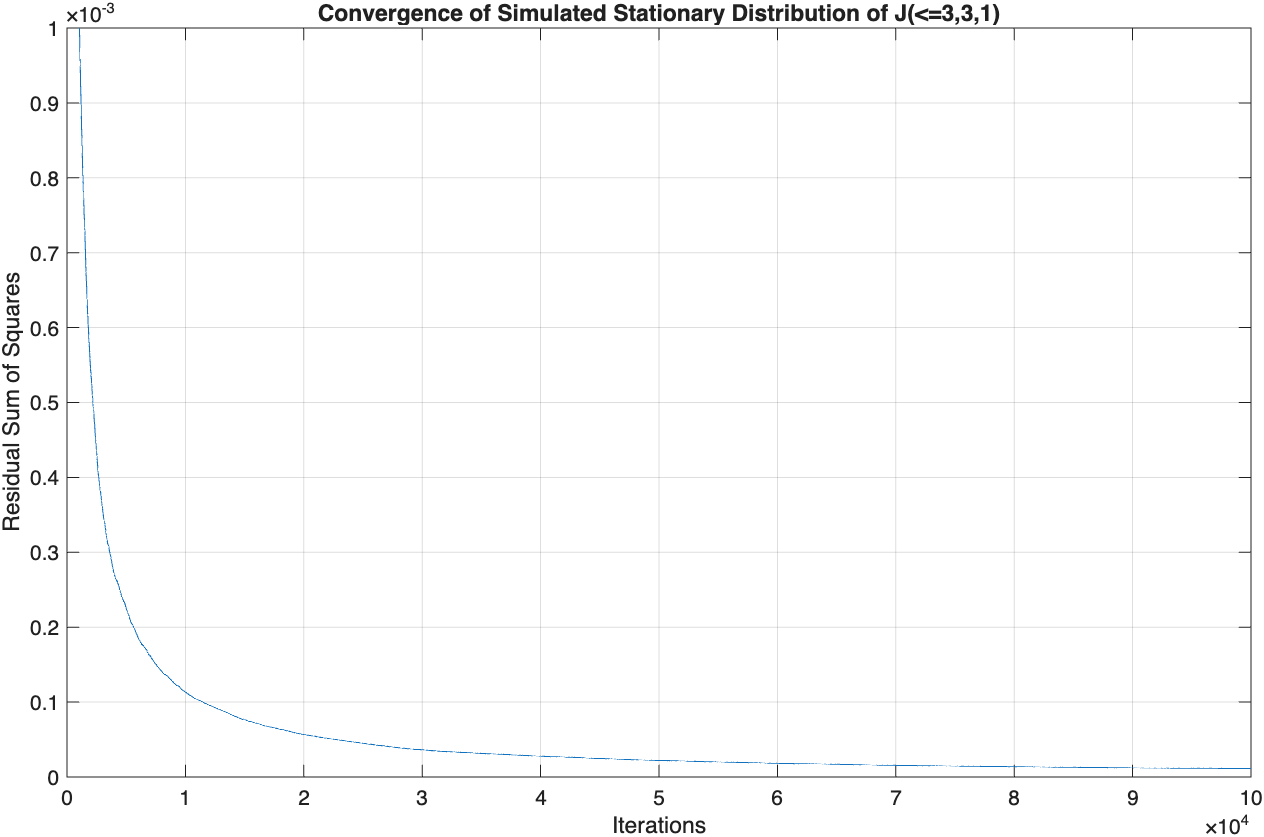
\includegraphics[width=1.0\linewidth]{images/convergence_1b3h.png}
%     \caption{Residual sum of squares plotted against number of iterations to show convergence of simulated stationary distribution with theoretical stationary state for juggling system  $J(\leq3,3,1)$}
%     \label{fig:convergence_1b3h}
% \end{figure}

% \begin{figure}[!htb]
%     \centering
%     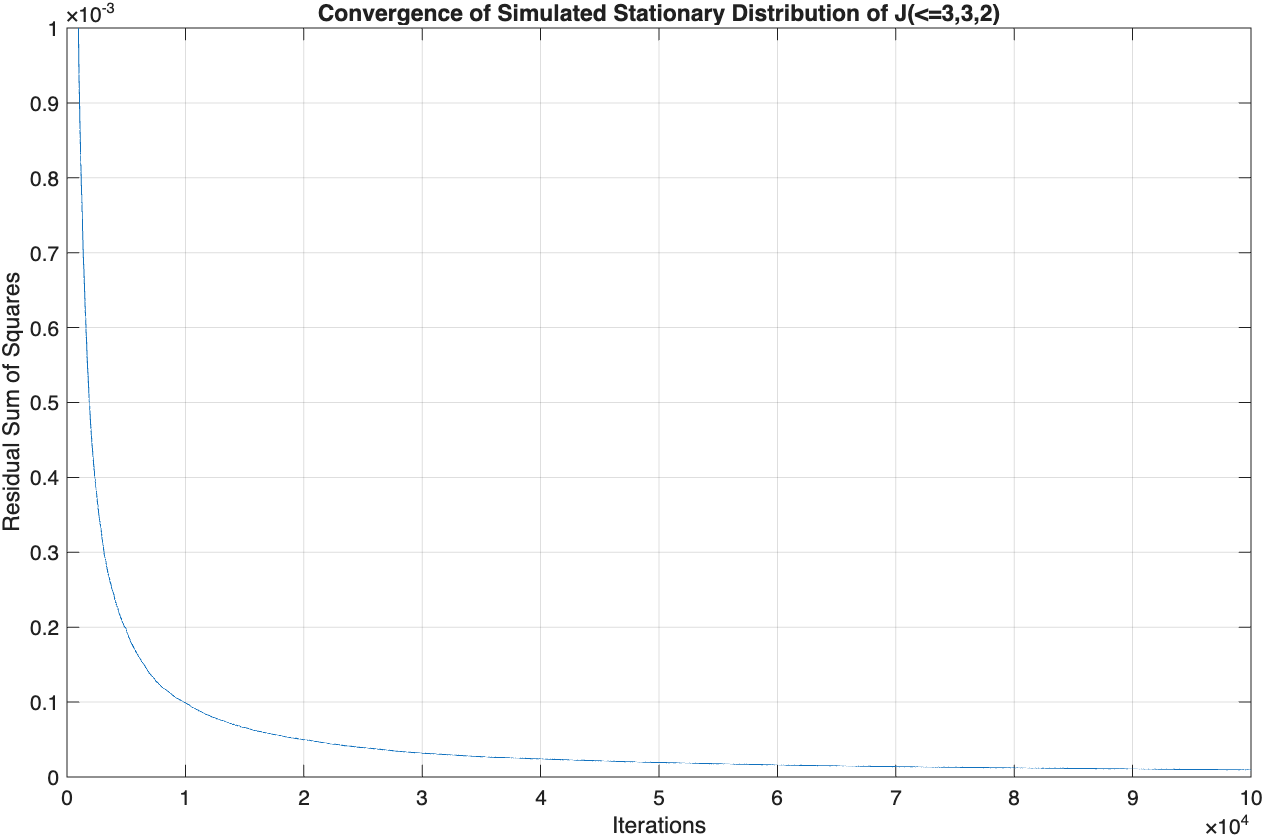
\includegraphics[width=1.0\linewidth]{images/convergence_2b3h.png}
%     \caption{Residual sum of squares plotted against number of iterations to show convergence of simulated stationary distribution with theoretical stationary state for juggling system  $J(\leq3,3,2)$}
%     \label{fig:convergence_2b3h}
% \end{figure}

\begin{figure}[!htb]
    \centering
    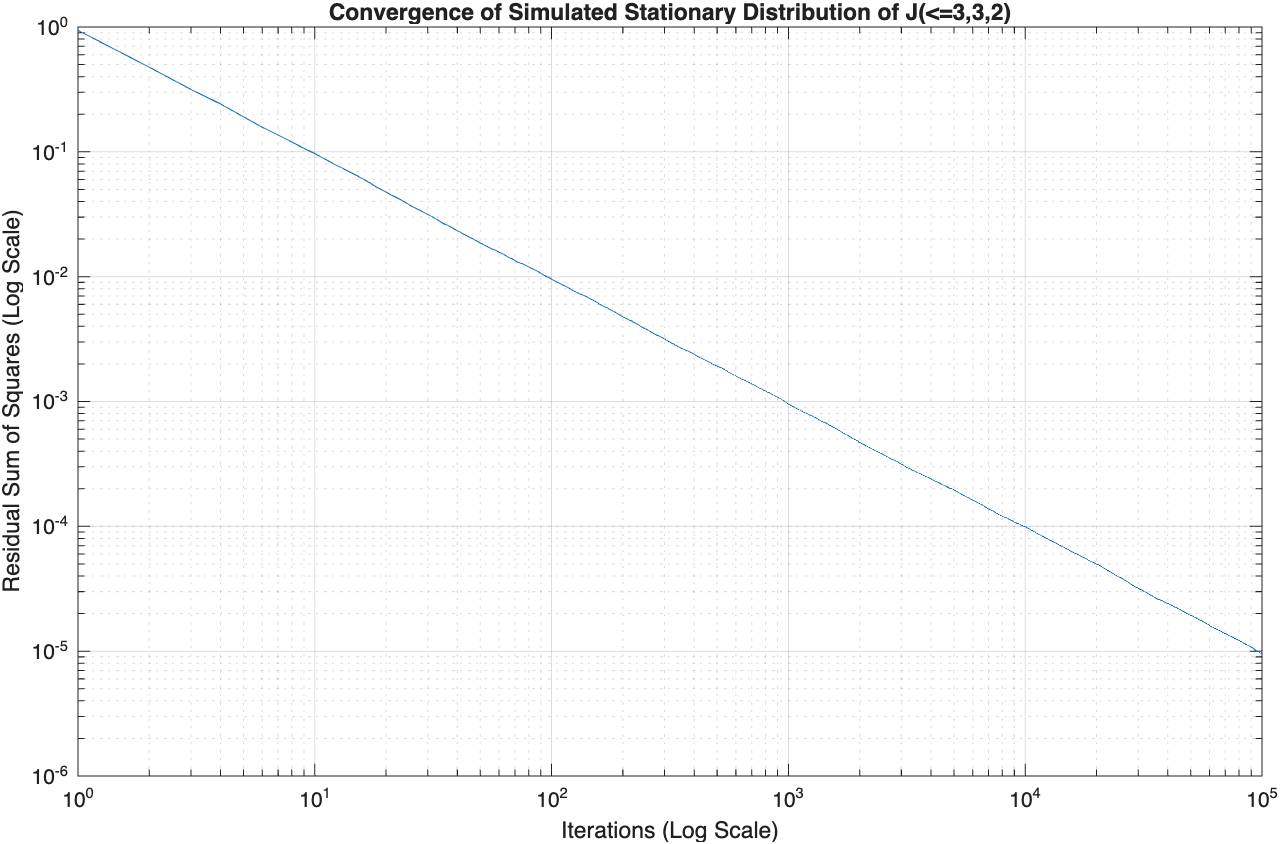
\includegraphics[width=1.0\linewidth]{images/logconvergence_2b3h.png}
    \caption{Residual sum of squares plotted against number of iterations to show convergence of simulated stationary distribution with theoretical stationary state for juggling system $J(\leq3,3,2)$ plotted on a log-log plot}
    \label{fig:logconvergence_2b3h}
\end{figure}

\begin{figure}[!htb]
    \centering
    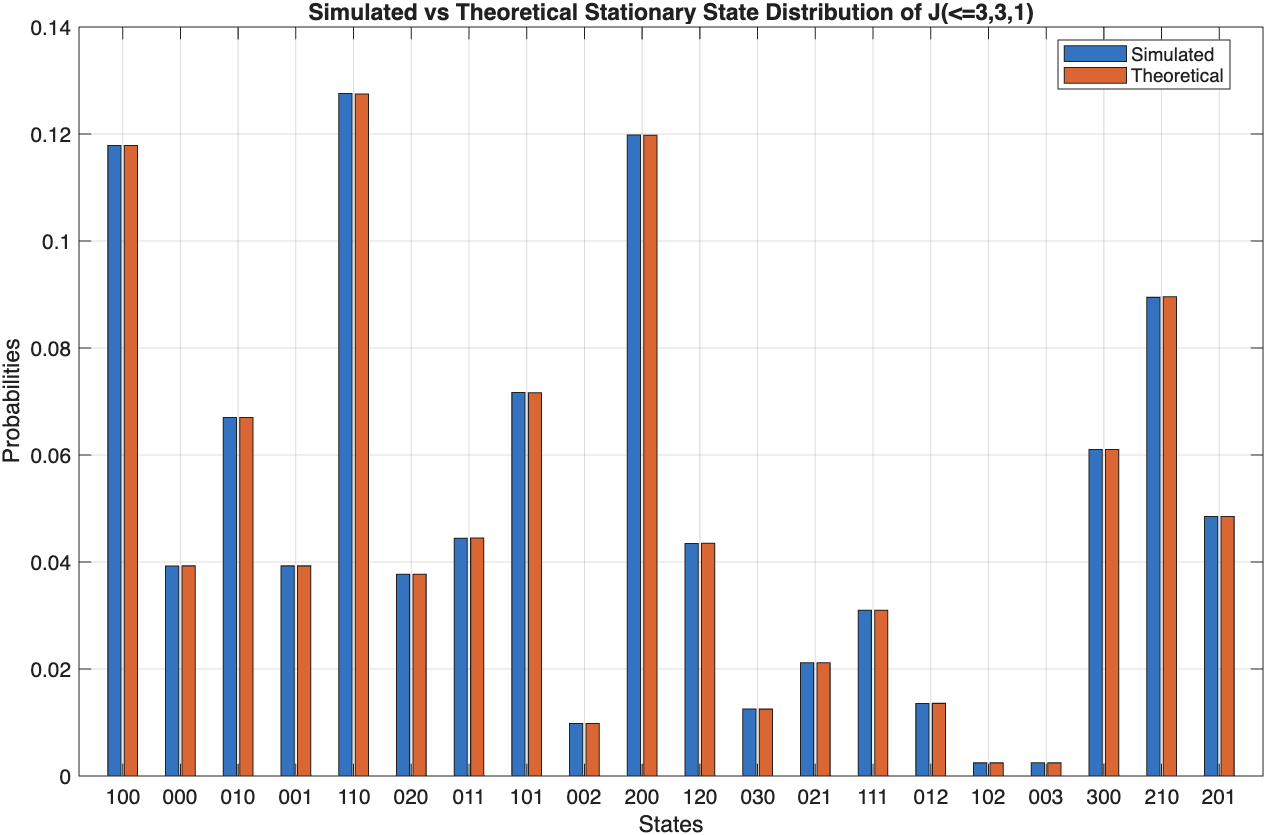
\includegraphics[width=1.0\linewidth]{images/sim_1b3h.png}
    \caption{Comparison of the probabilities of simulated stationary state (blue) against theoretical stationary state (red) for juggling system  $J(\leq3,3,1)$}
    \label{fig:sim_1b3h}
\end{figure}

\begin{figure}[!htb]
    \centering
    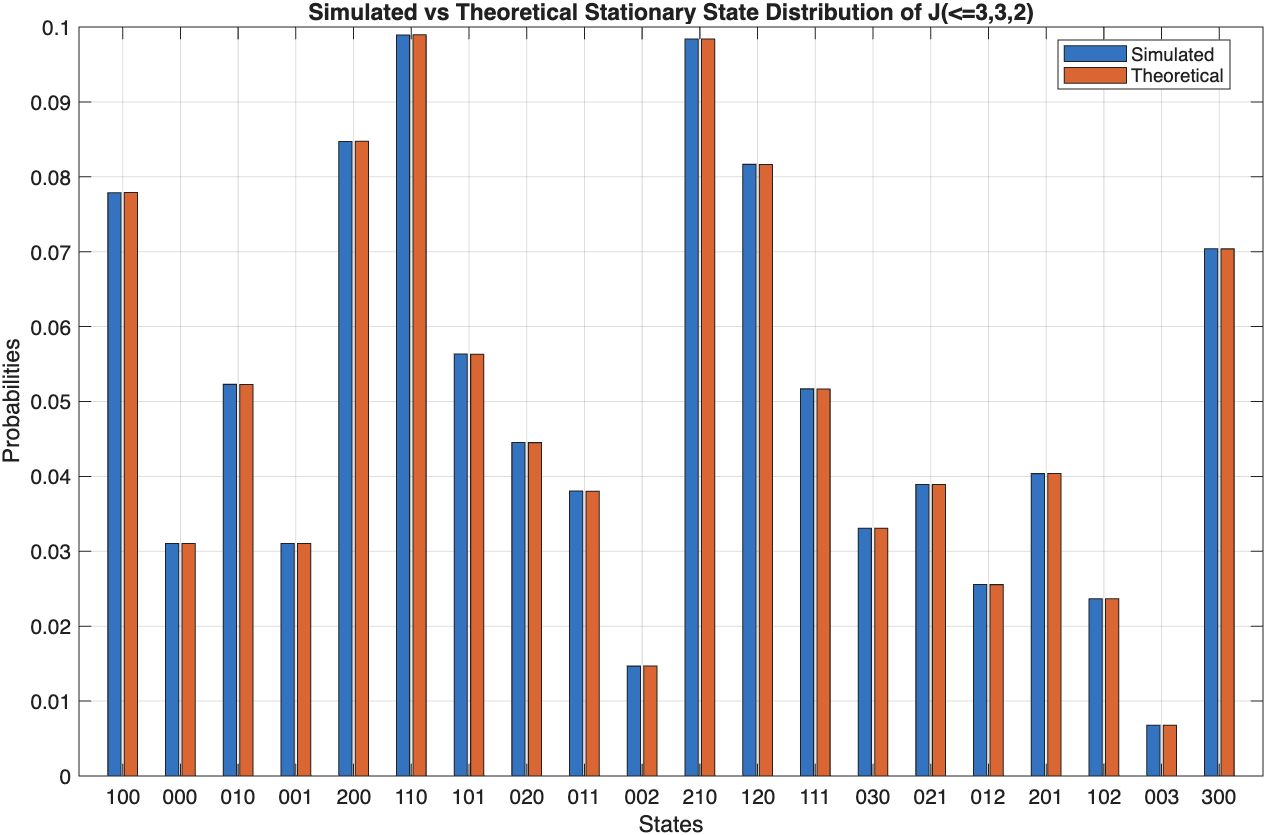
\includegraphics[width=1.0\linewidth]{images/sim_2b3h.png}
    \caption{Comparison of the probabilities of simulated stationary state (blue) against theoretical stationary state (red) for juggling system  $J(\leq3,3,2)$}
    \label{fig:sim_2b3h}
\end{figure}

% \begin{figure}[!htb]
%     \centering
%     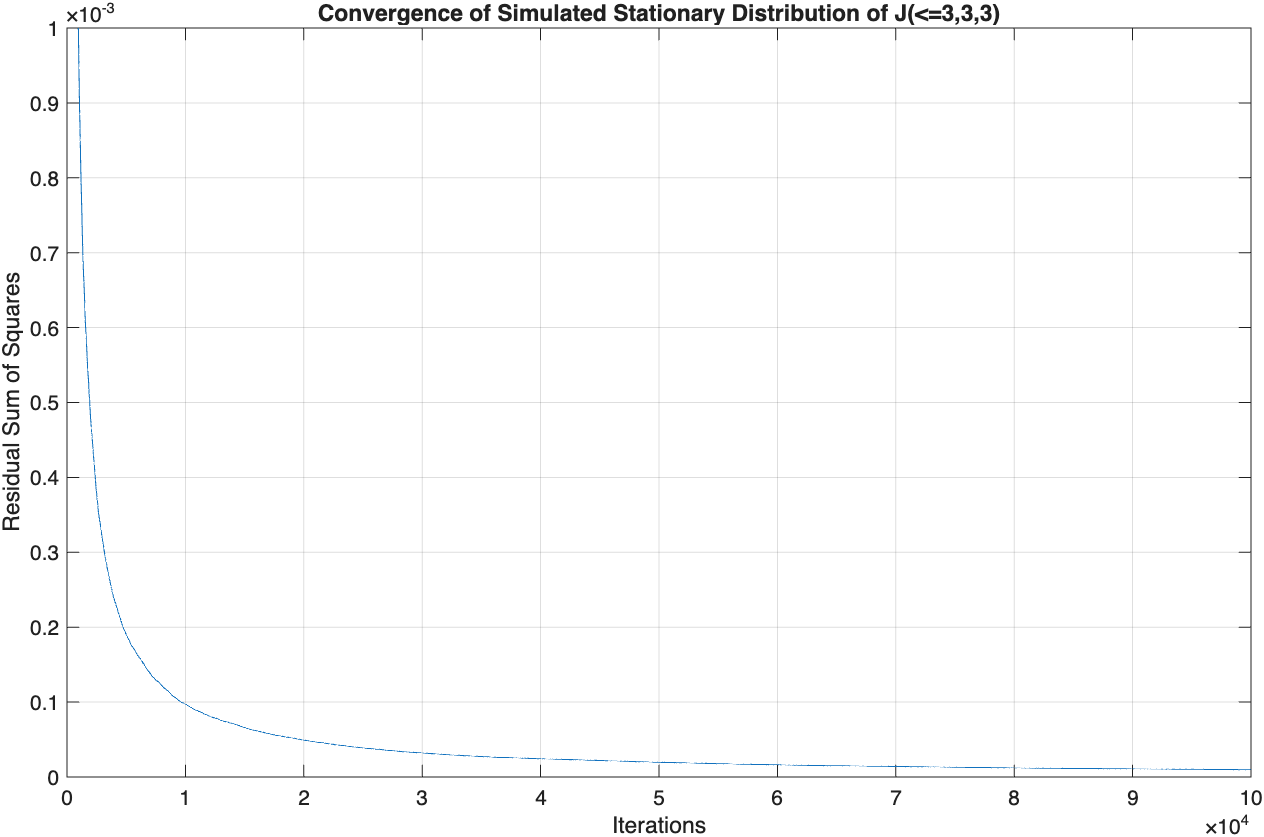
\includegraphics[width=1.0\linewidth]{images/convergence_3b3h.png}
%     \caption{Residual sum of squares plotted against number of iterations to show convergence of simulated stationary distribution with theoretical stationary state for juggling system  $J(\leq3,3,3)$}
%     \label{fig:convergence_3b3h}
% \end{figure}

\begin{figure}[!htb]
    \centering
    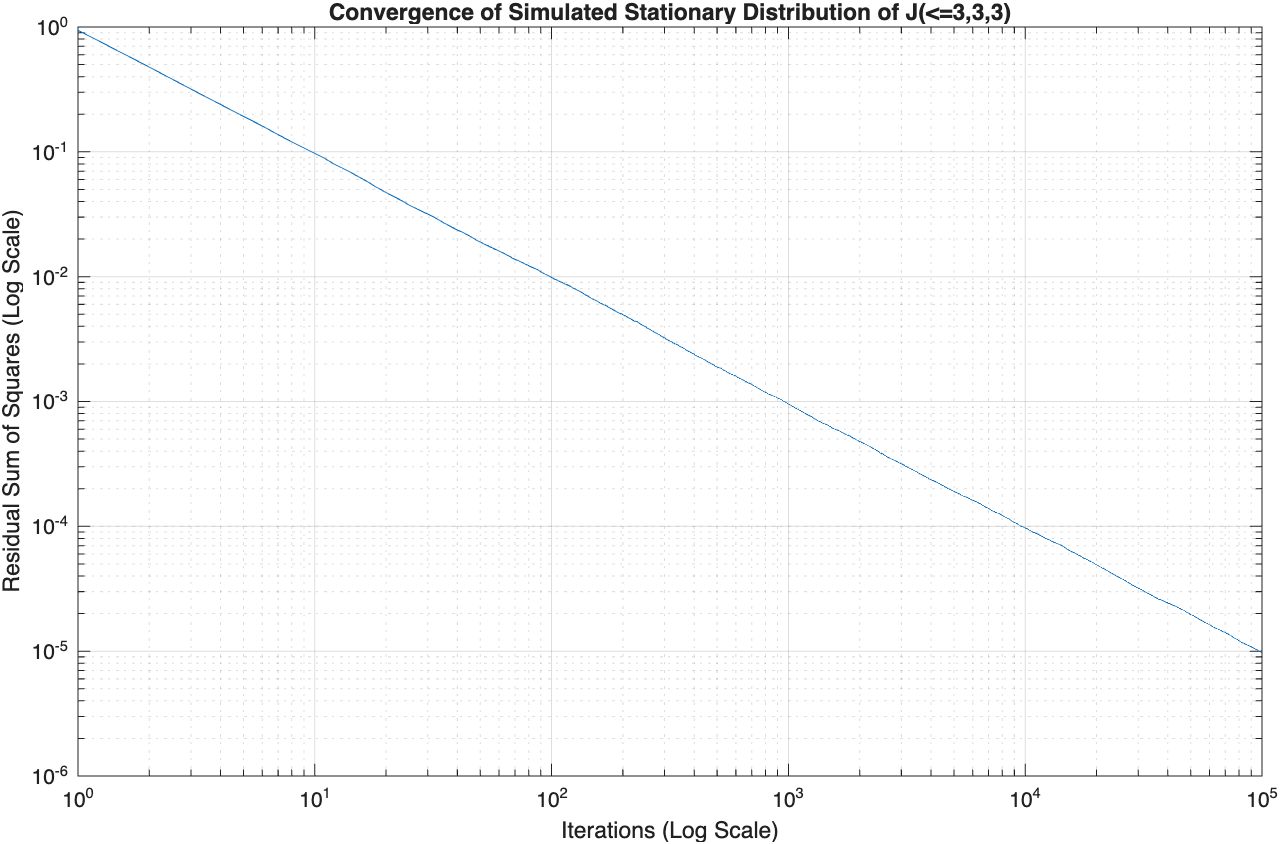
\includegraphics[width=1.0\linewidth]{images/logconvergence_3b3h.png}
    \caption{Residual sum of squares plotted against number of iterations to show convergence of simulated stationary distribution with theoretical stationary state for juggling system $J(\leq3,3,3)$ plotted on a log-log plot}
    \label{fig:logconvergence_3b3h}
\end{figure}



\begin{figure}[!htb]
    \centering
    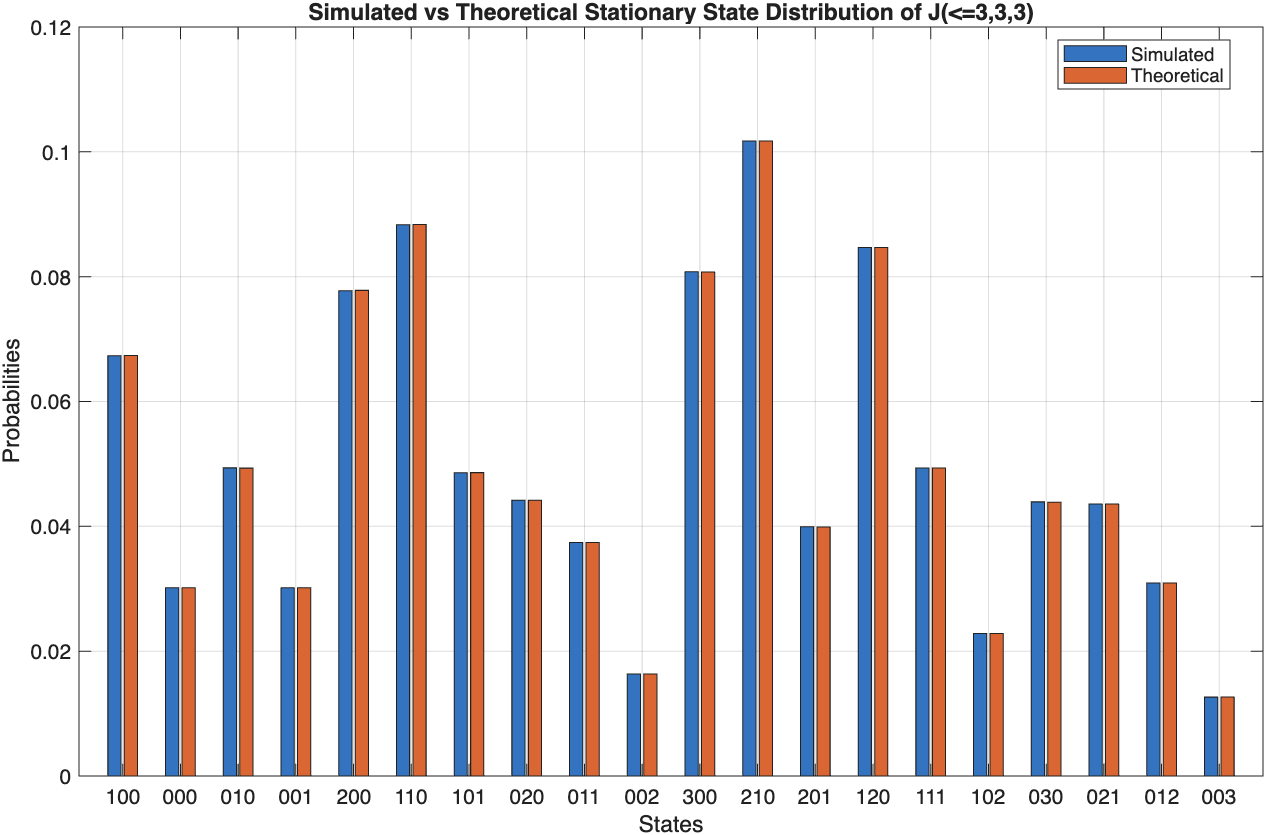
\includegraphics[width=1.0\linewidth]{images/sim_3b3h.png}
    \caption{Comparison of the probabilities of simulated stationary state (blue) against theoretical stationary state (red) for juggling system  $J(\leq3,6,3)$}
    \label{fig:sim_3b3h}
\end{figure}

% \begin{figure}[!htb]
%     \centering
%     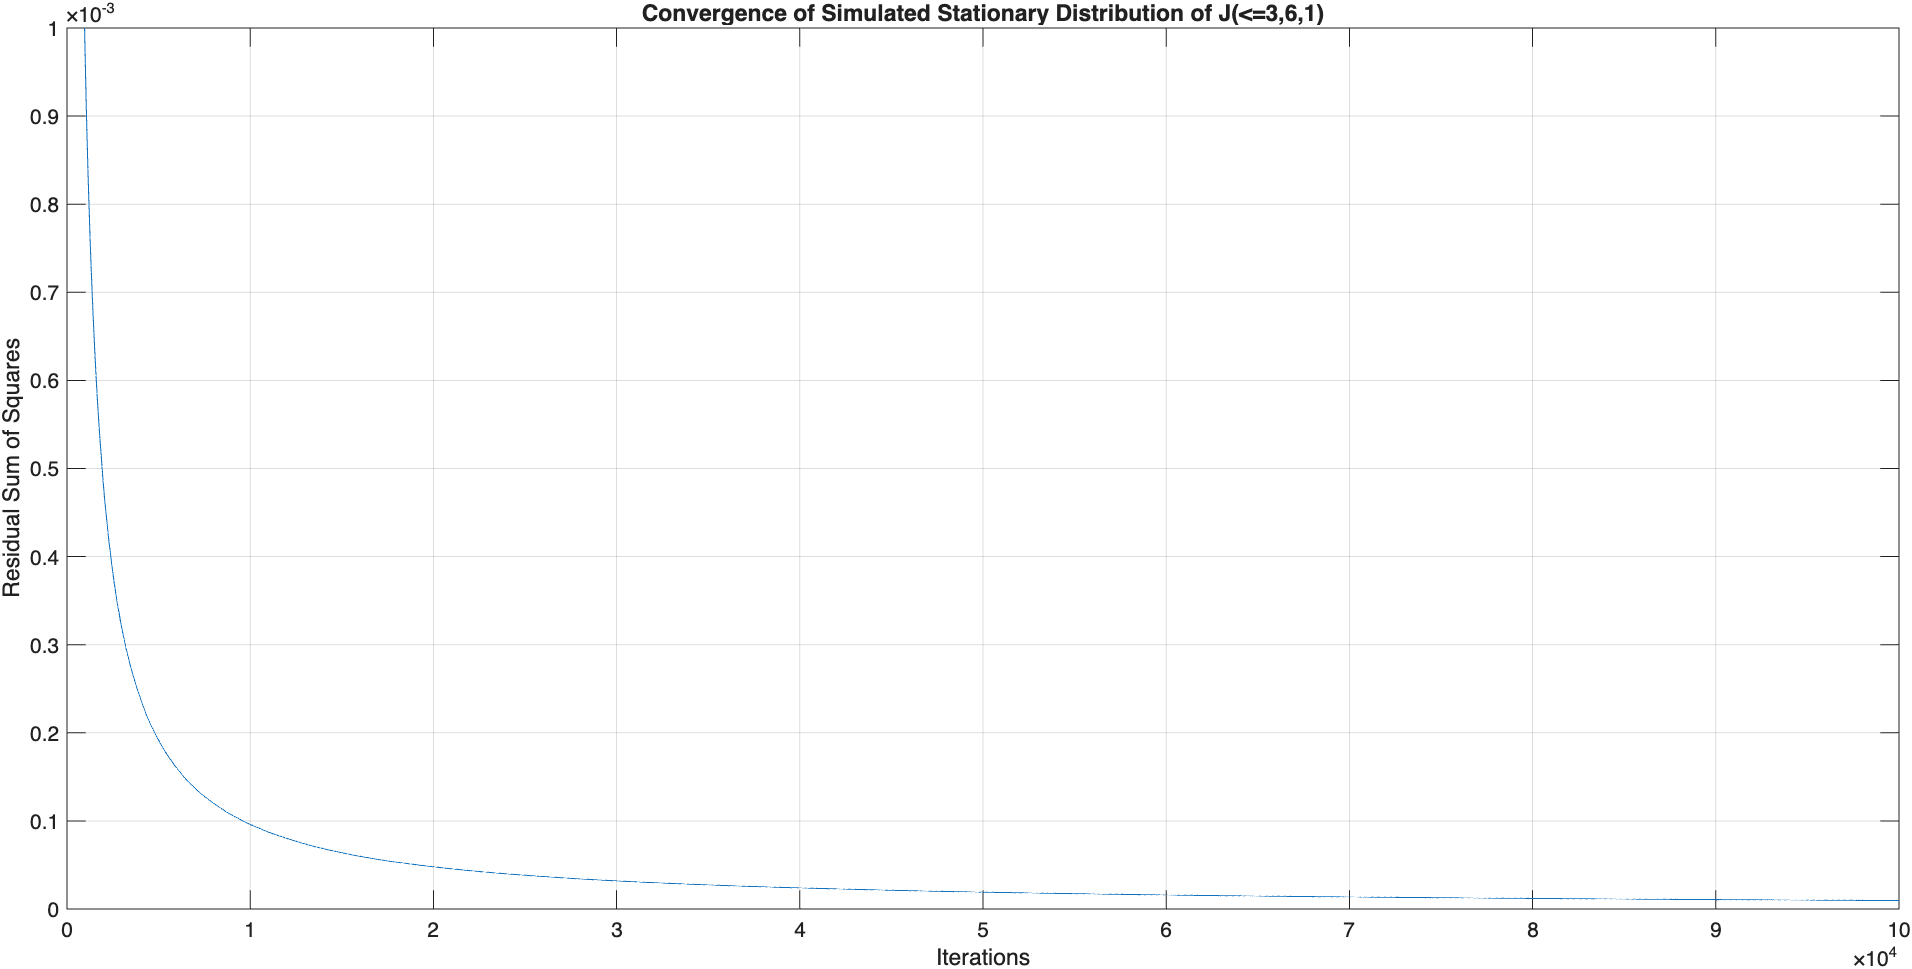
\includegraphics[width=1.0\linewidth]{images/convergence_1b6h.png}
%     \caption{Residual sum of squares plotted against number of iterations to show convergence of simulated stationary distribution with theoretical stationary state for juggling system  $J(\leq3,6,1)$}
%     \label{fig:convergence_1b6h}
% \end{figure}

\begin{figure}[!htb]
    \centering
    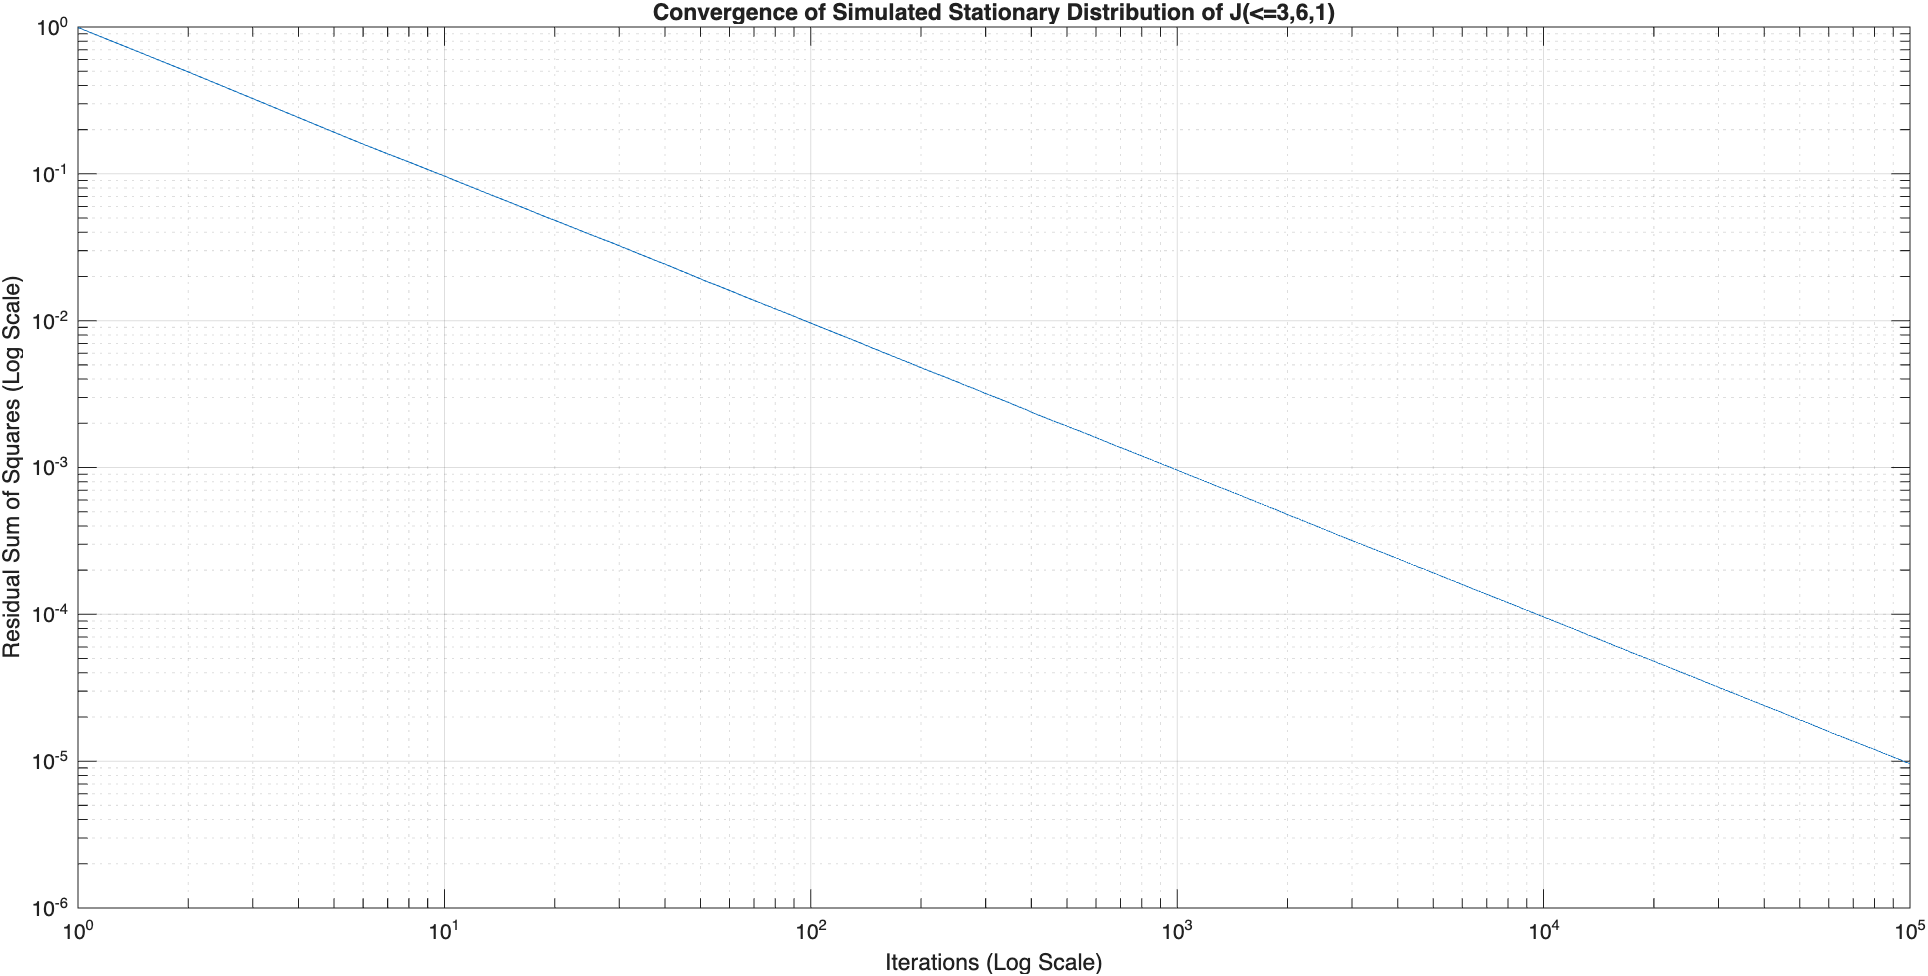
\includegraphics[width=1.0\linewidth]{images/logconvergence_1b6h.png}
    \caption{Residual sum of squares plotted against number of iterations to show convergence of simulated stationary distribution with theoretical stationary state for juggling system $J(\leq3,6,1)$ plotted on a log-log plot}
    \label{fig:logconvergence_1b6h}
\end{figure}

\begin{figure}[!htb]
    \centering
    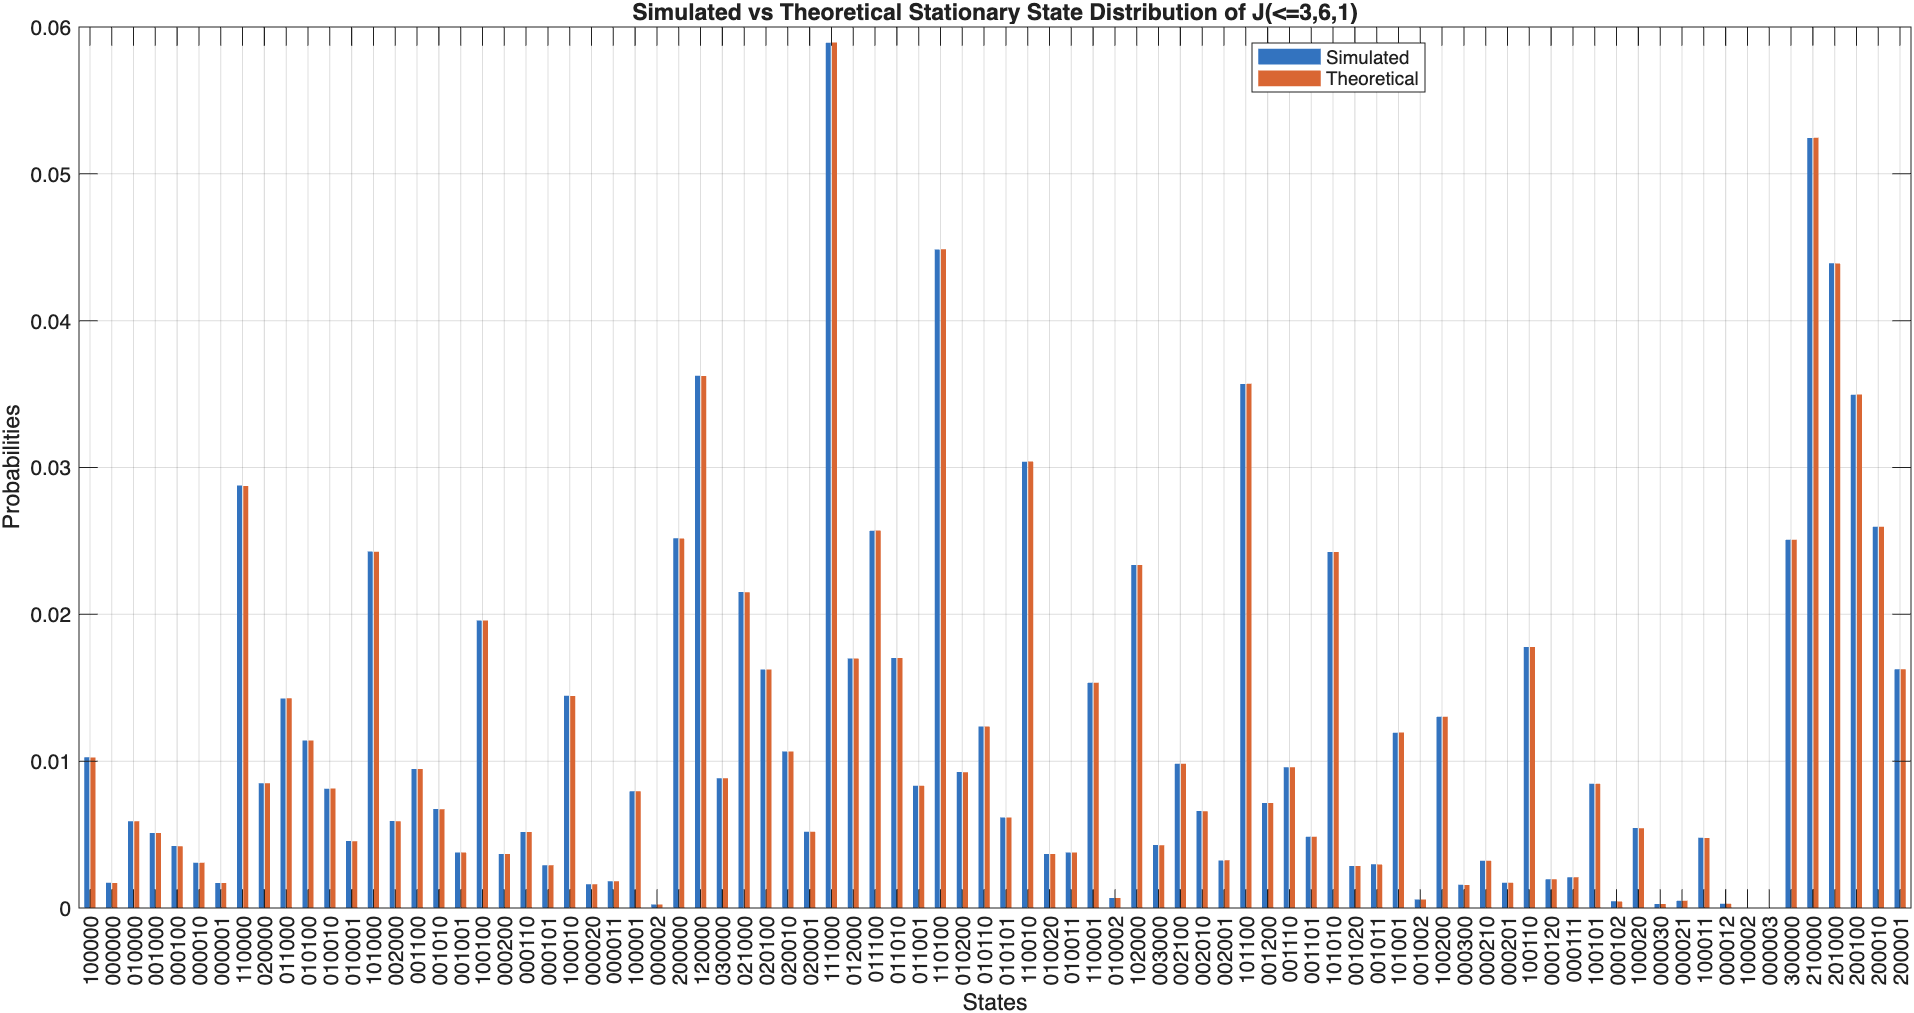
\includegraphics[width=1.0\linewidth]{images/sim_1b6h.png}
    \caption{Comparison of the probabilities of simulated stationary state (blue) against theoretical stationary state (red) for juggling system  $J(\leq3,3,1)$}
    \label{fig:sim_1b6h}
\end{figure}


\subsection{Simulation: Results from Terminal} \label{sec:terminal}
\begin{figure}[!htb]
    \centering
    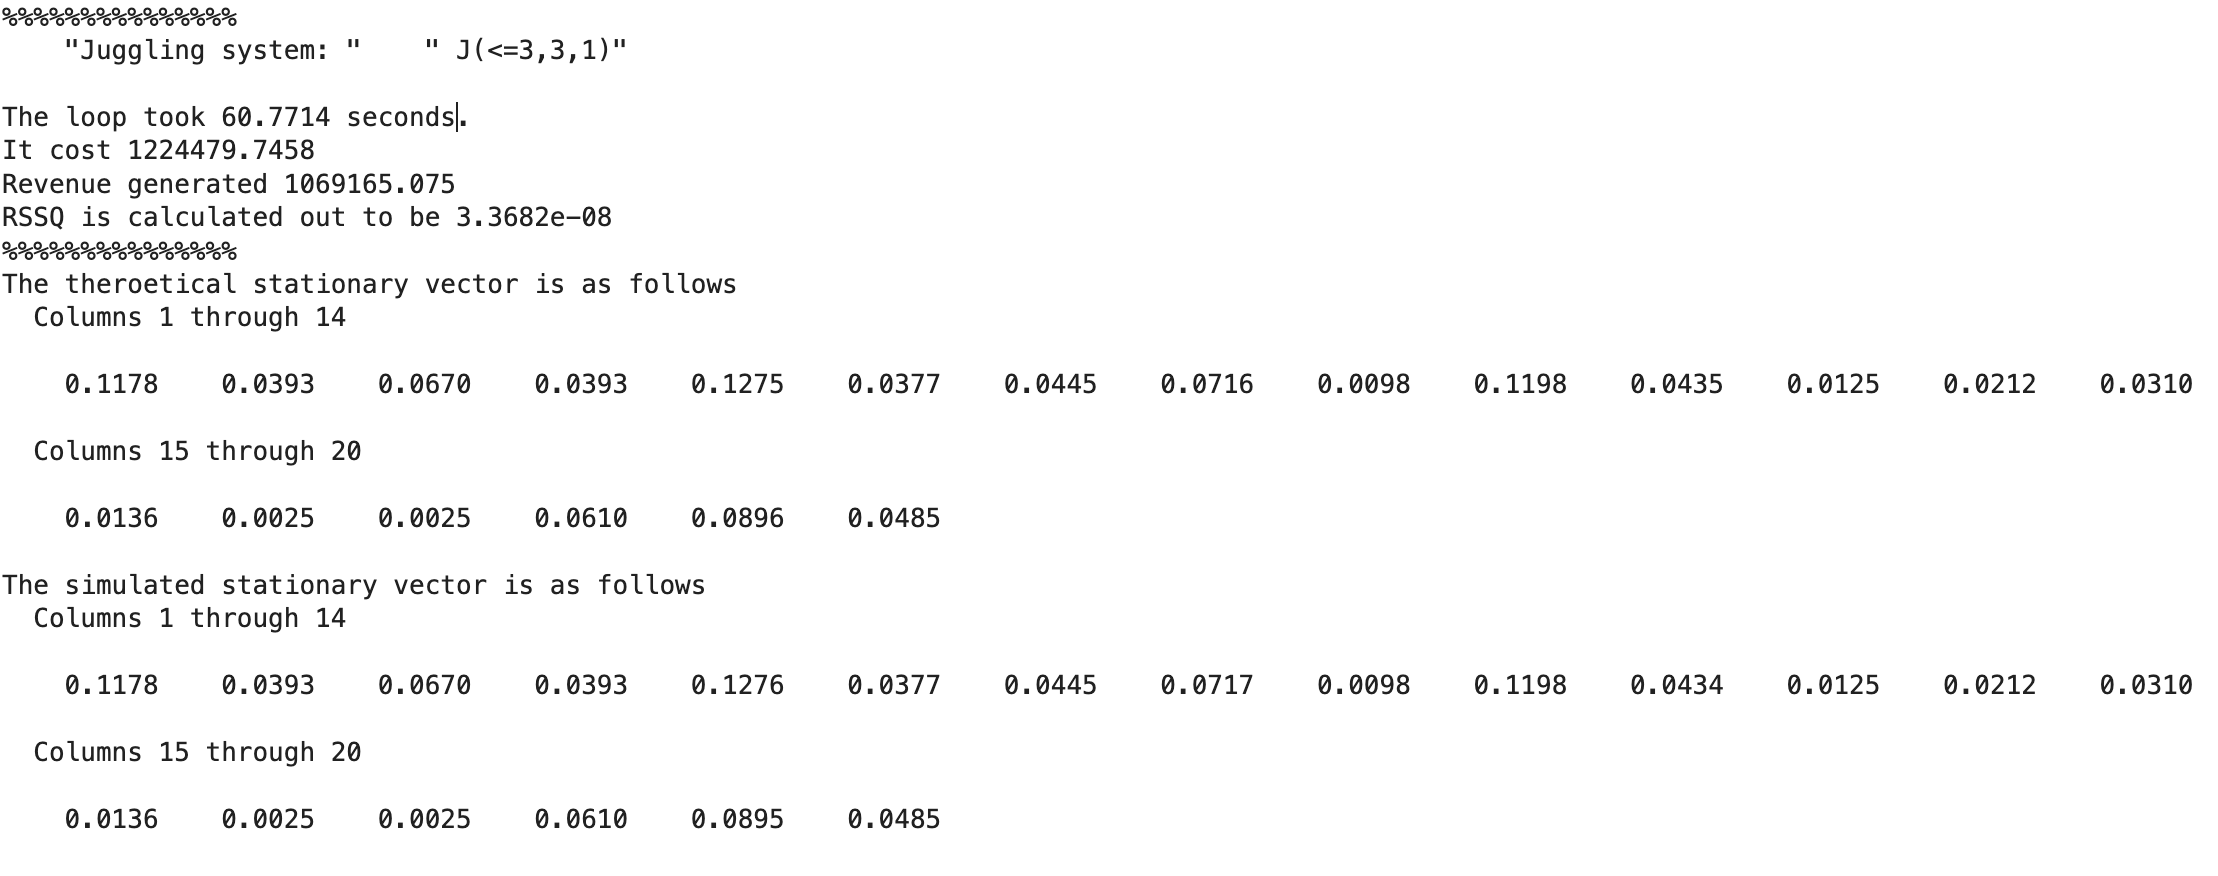
\includegraphics[width=1.0\linewidth]{images/terminal_1b3h.png}
    \caption{Terminal output showing run time, economic values, rssq and theoretical and simulated stationary state vectors for $J(\leq3,3,1)$}
    \label{fig:terminal_1b3h}
\end{figure}

\begin{figure}[!htb]
    \centering
    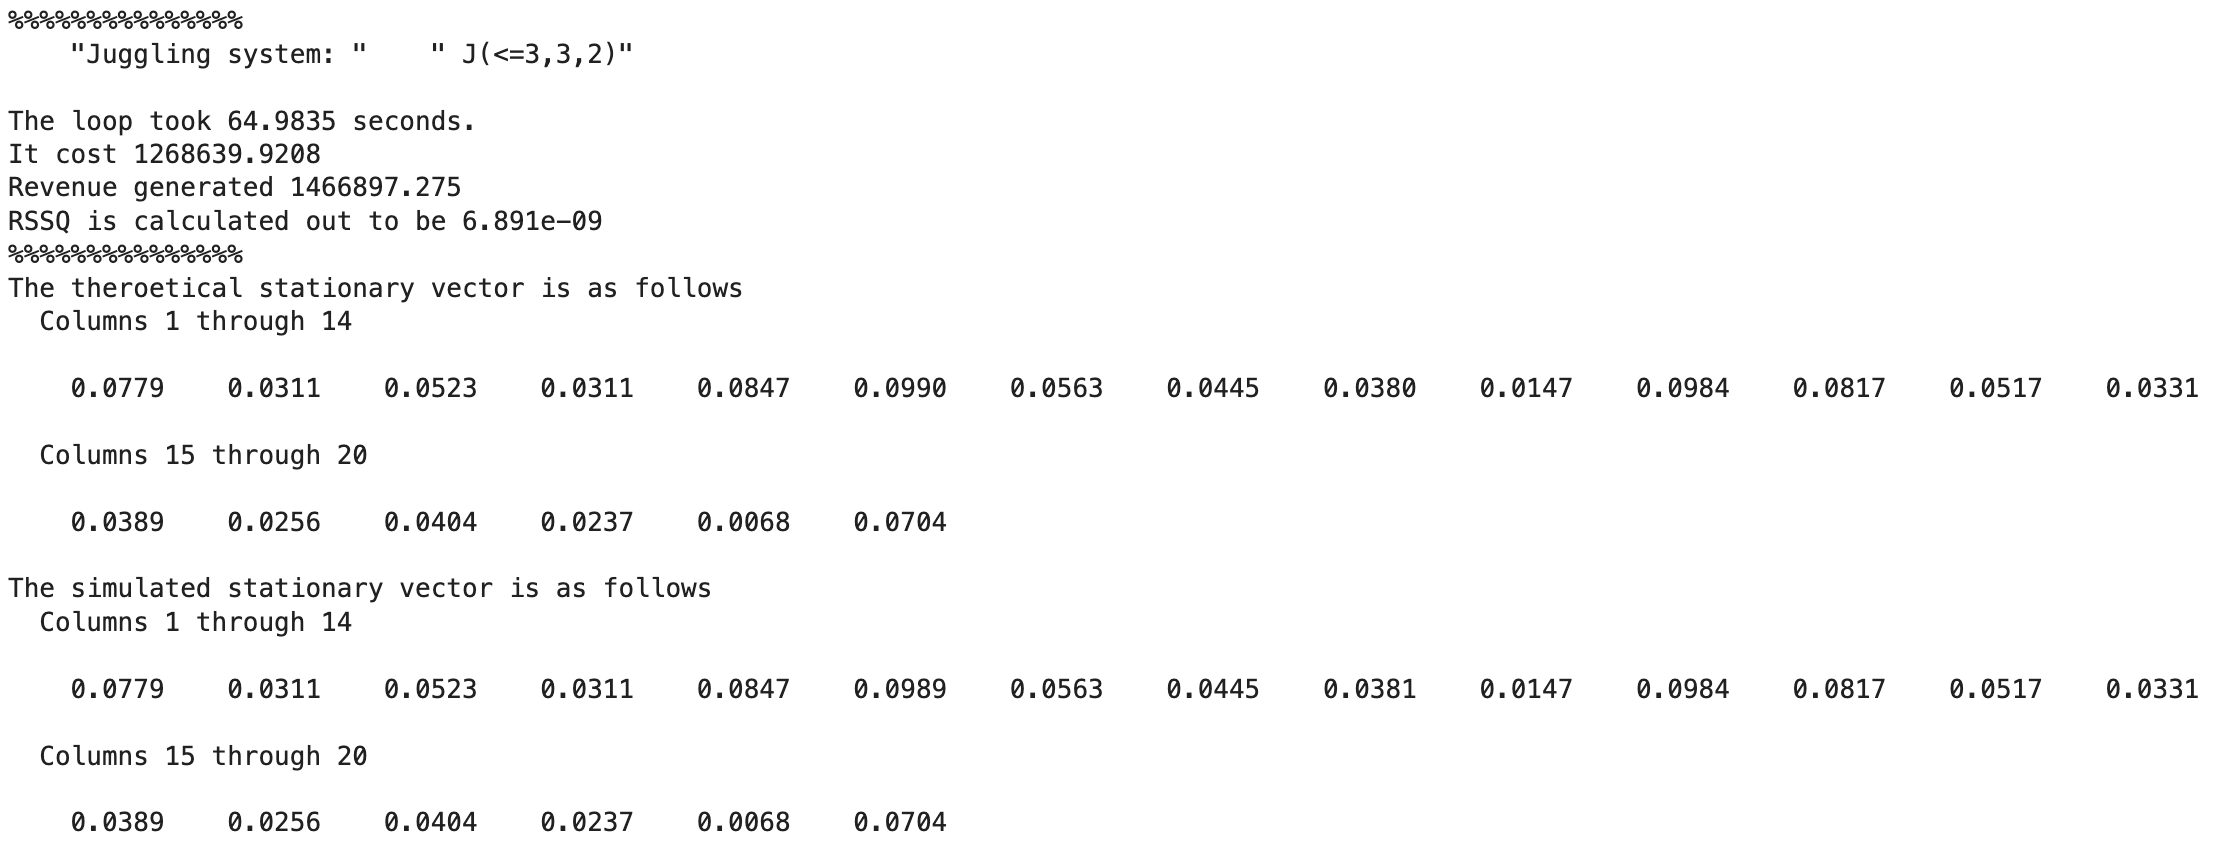
\includegraphics[width=1.0\linewidth]{images/terminal_2b3h.png}
    \caption{Terminal output showing run time, economic values, rssq and theoretical and simulated stationary state vectors for $J(\leq3,3,2)$}
    \label{fig:terminal_2b3h}
\end{figure}

\begin{figure}[!htb]
    \centering
    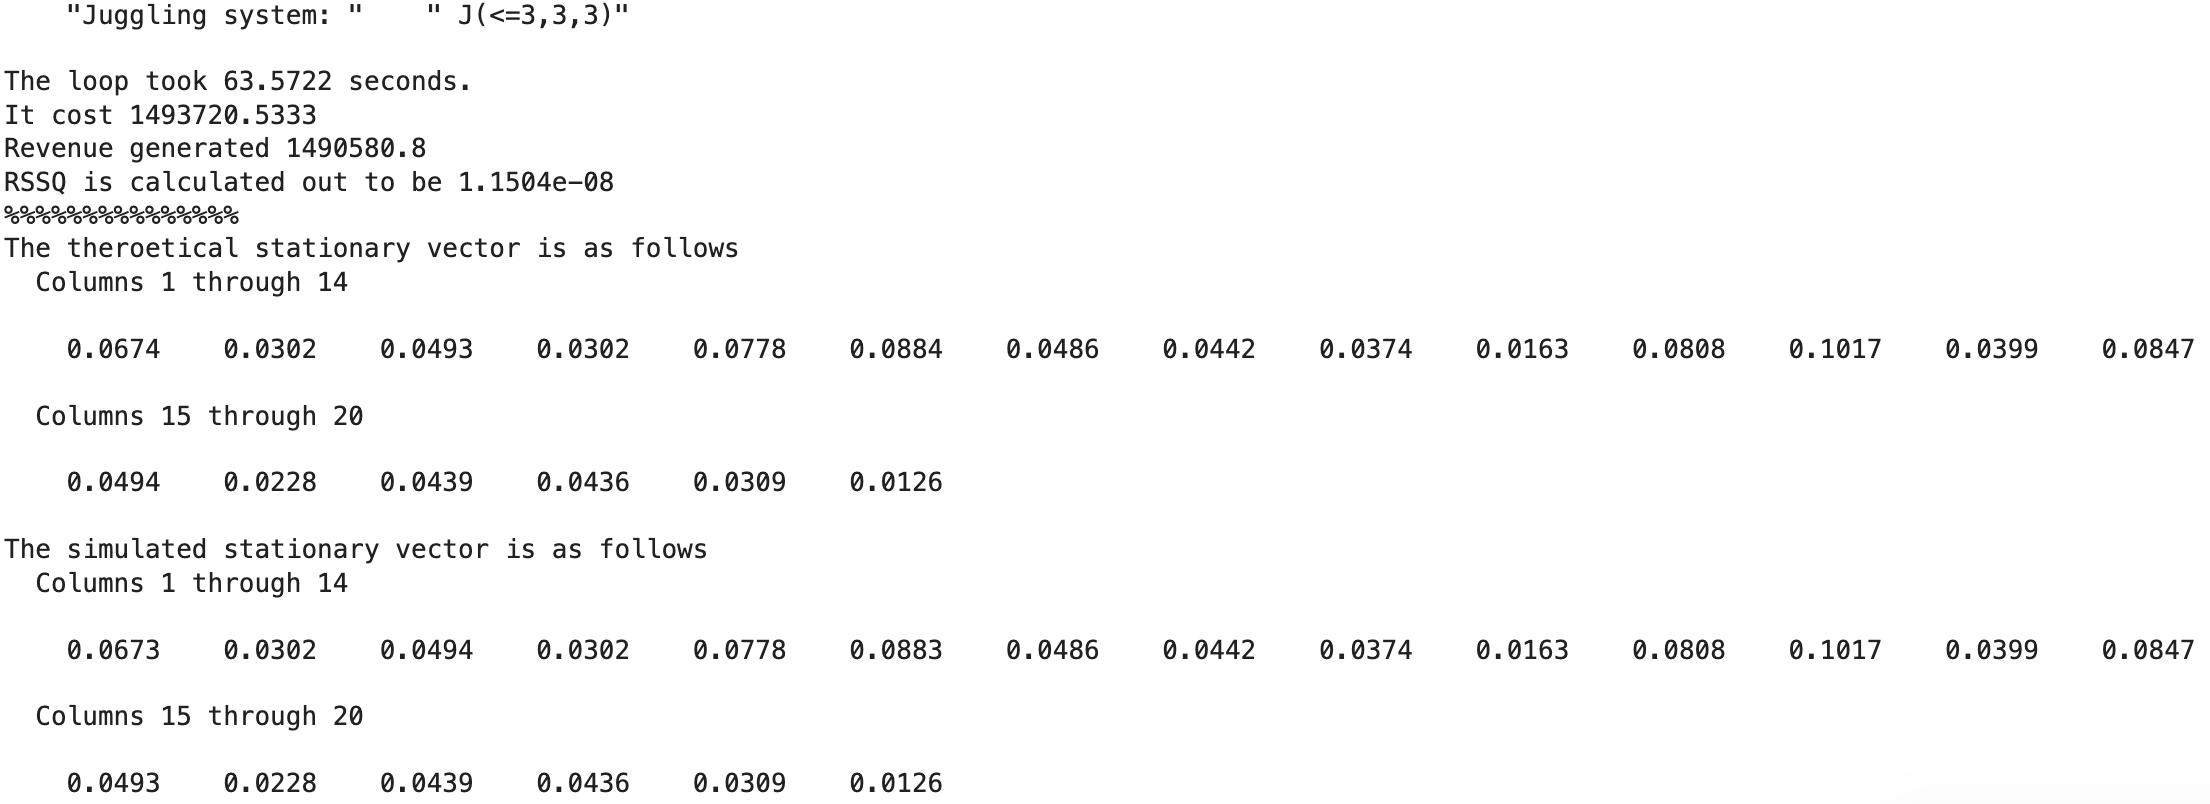
\includegraphics[width=1.0\linewidth]{images/terminal_3b3h.png}
    \caption{Terminal output showing run time, economic values, rssq and theoretical and simulated stationary state vectors for $J(\leq3,3,3)$}
    \label{fig:terminal_3b3h}
\end{figure}


\begin{figure}[!htb]
    \centering
    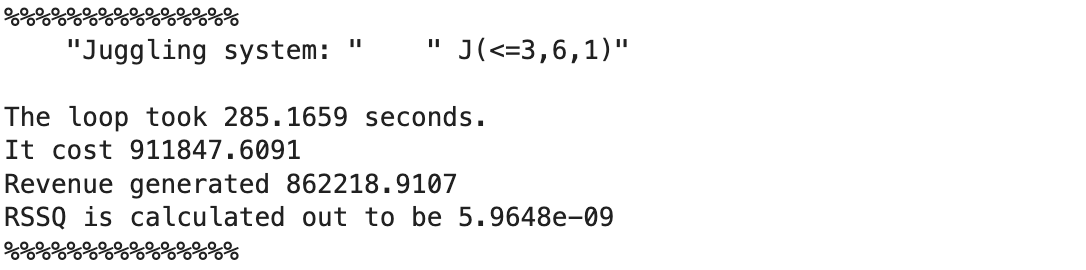
\includegraphics[width=1.0\linewidth]{images/terminal_1b6h_i.png}
    \caption{Terminal output showing run time, economic values, rssq and theoretical and simulated stationary state vectors for $J(\leq3,6,1)$}
    \label{fig:terminal_1b6h_i}
\end{figure}

\begin{figure}[!htb]
    \centering
    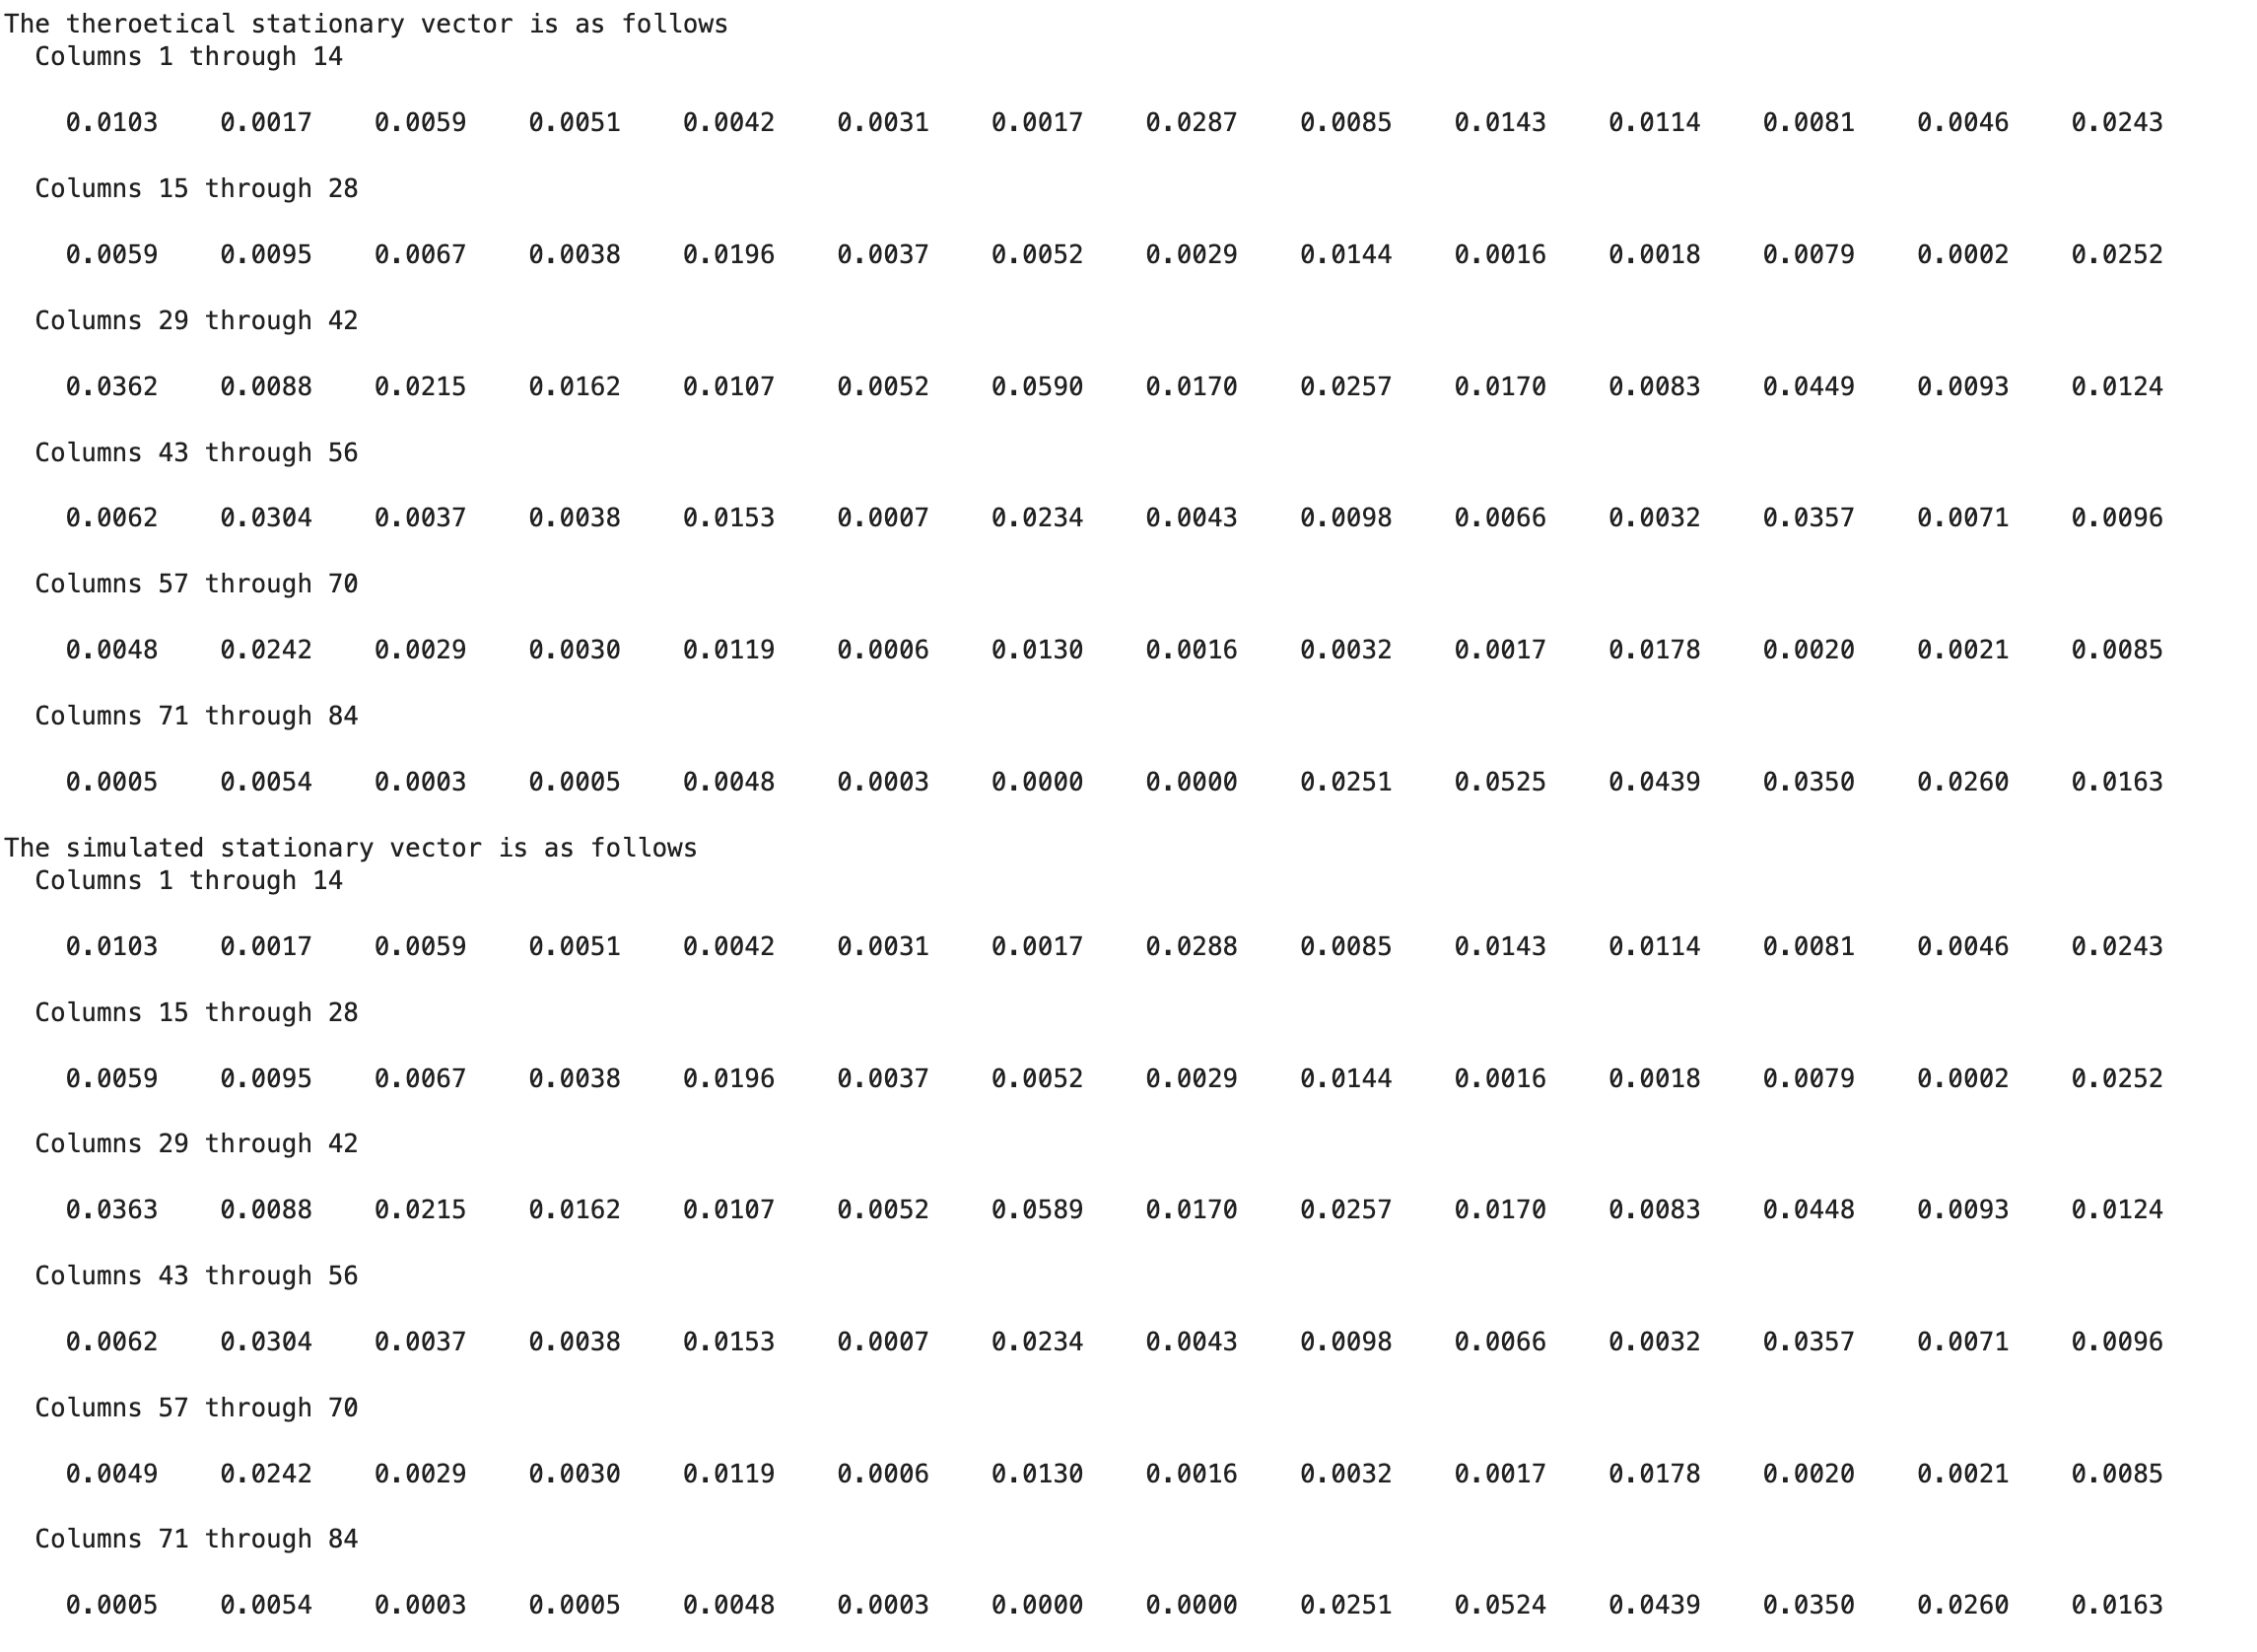
\includegraphics[width=1.0\linewidth]{images/terminal_1b6h_ii.png}
    \caption{Comparison of the probabilities of simulated stationary state (blue) against theoretical stationary state (red) for juggling system  $J(\leq3,6,1)$}
    \label{fig:terminal_1b6h_ii}
\end{figure}

\subsection{Economic Results}
These values have been extracted and collected from output images in the terminal section \ref{sec:terminal} above 
\begin{table}[!htb]
    \centering
    \begin{tabular}{|l|c|c|c|c|}
         \hline
         & Exp 1 & Exp 2 & Exp 3 & Exp 4 \\ \hline
        Run Time    & 60.01        & 66.44        & 63.09       & 261.73     \\ \hline
        Avg Cost    & 1,224,479.75 & 1,268,639.92 & 1,493,720.53 & 911,847.61 \\ \hline
        Avg Revenue & 1,069,165.08 & 1,466,897.28 & 1,490,580.80 & 862,218.91 \\ \hline
        Avg Profit  & (155,314.67) & 198,257.35   & (3,139.73)   & (49,628.70) \\ \hline
        \end{tabular}
        \caption{Comparing the run time, average revenue, average cost and average profit with different number of bays and throw heights}
        \label{tab:simrun}
\end{table}

\end{document}






